\documentclass[a4paper]{article}

\usepackage[english]{babel}
\usepackage[T1]{fontenc}
\usepackage{amsmath}
\usepackage{graphicx}
\usepackage[colorinlistoftodos]{todonotes}
\usepackage{makeidx}
\usepackage{fullpage,xspace,setspace,lscape}
\makeindex

\renewcommand{\thefigure}{S\arabic{figure}}


\title{\huge\bfseries \vspace{2cm} The \textit{E. coli} molecular phenotype under different growth conditions \\ \vspace{0.7cm}
	\Large\bfseries Supplementary materials \vspace{1.3cm}}


\author{
	\large\bfseries Mehmet U. Caglar*, John R. Houser, Craig S. Barnhart, \\
	\large\bfseries Daniel R. Boutz, Sean M. Carroll, Aurko Dasgupta, Walter F. Lenoir,\\ 
	\large\bfseries Bartram L. Smith, Viswanadham Sridhara, Dariya K. Sydykova, \\
	\large\bfseries Drew Vander Wood, Christopher J. Marx, \\
	\large\bfseries Edward M. Marcotte*, Jeffrey E. Barrick*, Claus O. Wilke*}


% allow floats to take up as much space as they want on a page
\renewcommand{\topfraction}{1.}	% max fraction of floats at top
\renewcommand{\bottomfraction}{1.}
\renewcommand{\textfraction}{0.}

\begin{document}
\maketitle
\newpage
	

\listoffigures


\newpage

\section*{Supplementary Figures}

\begin{figure}[!htb]
\centerline{	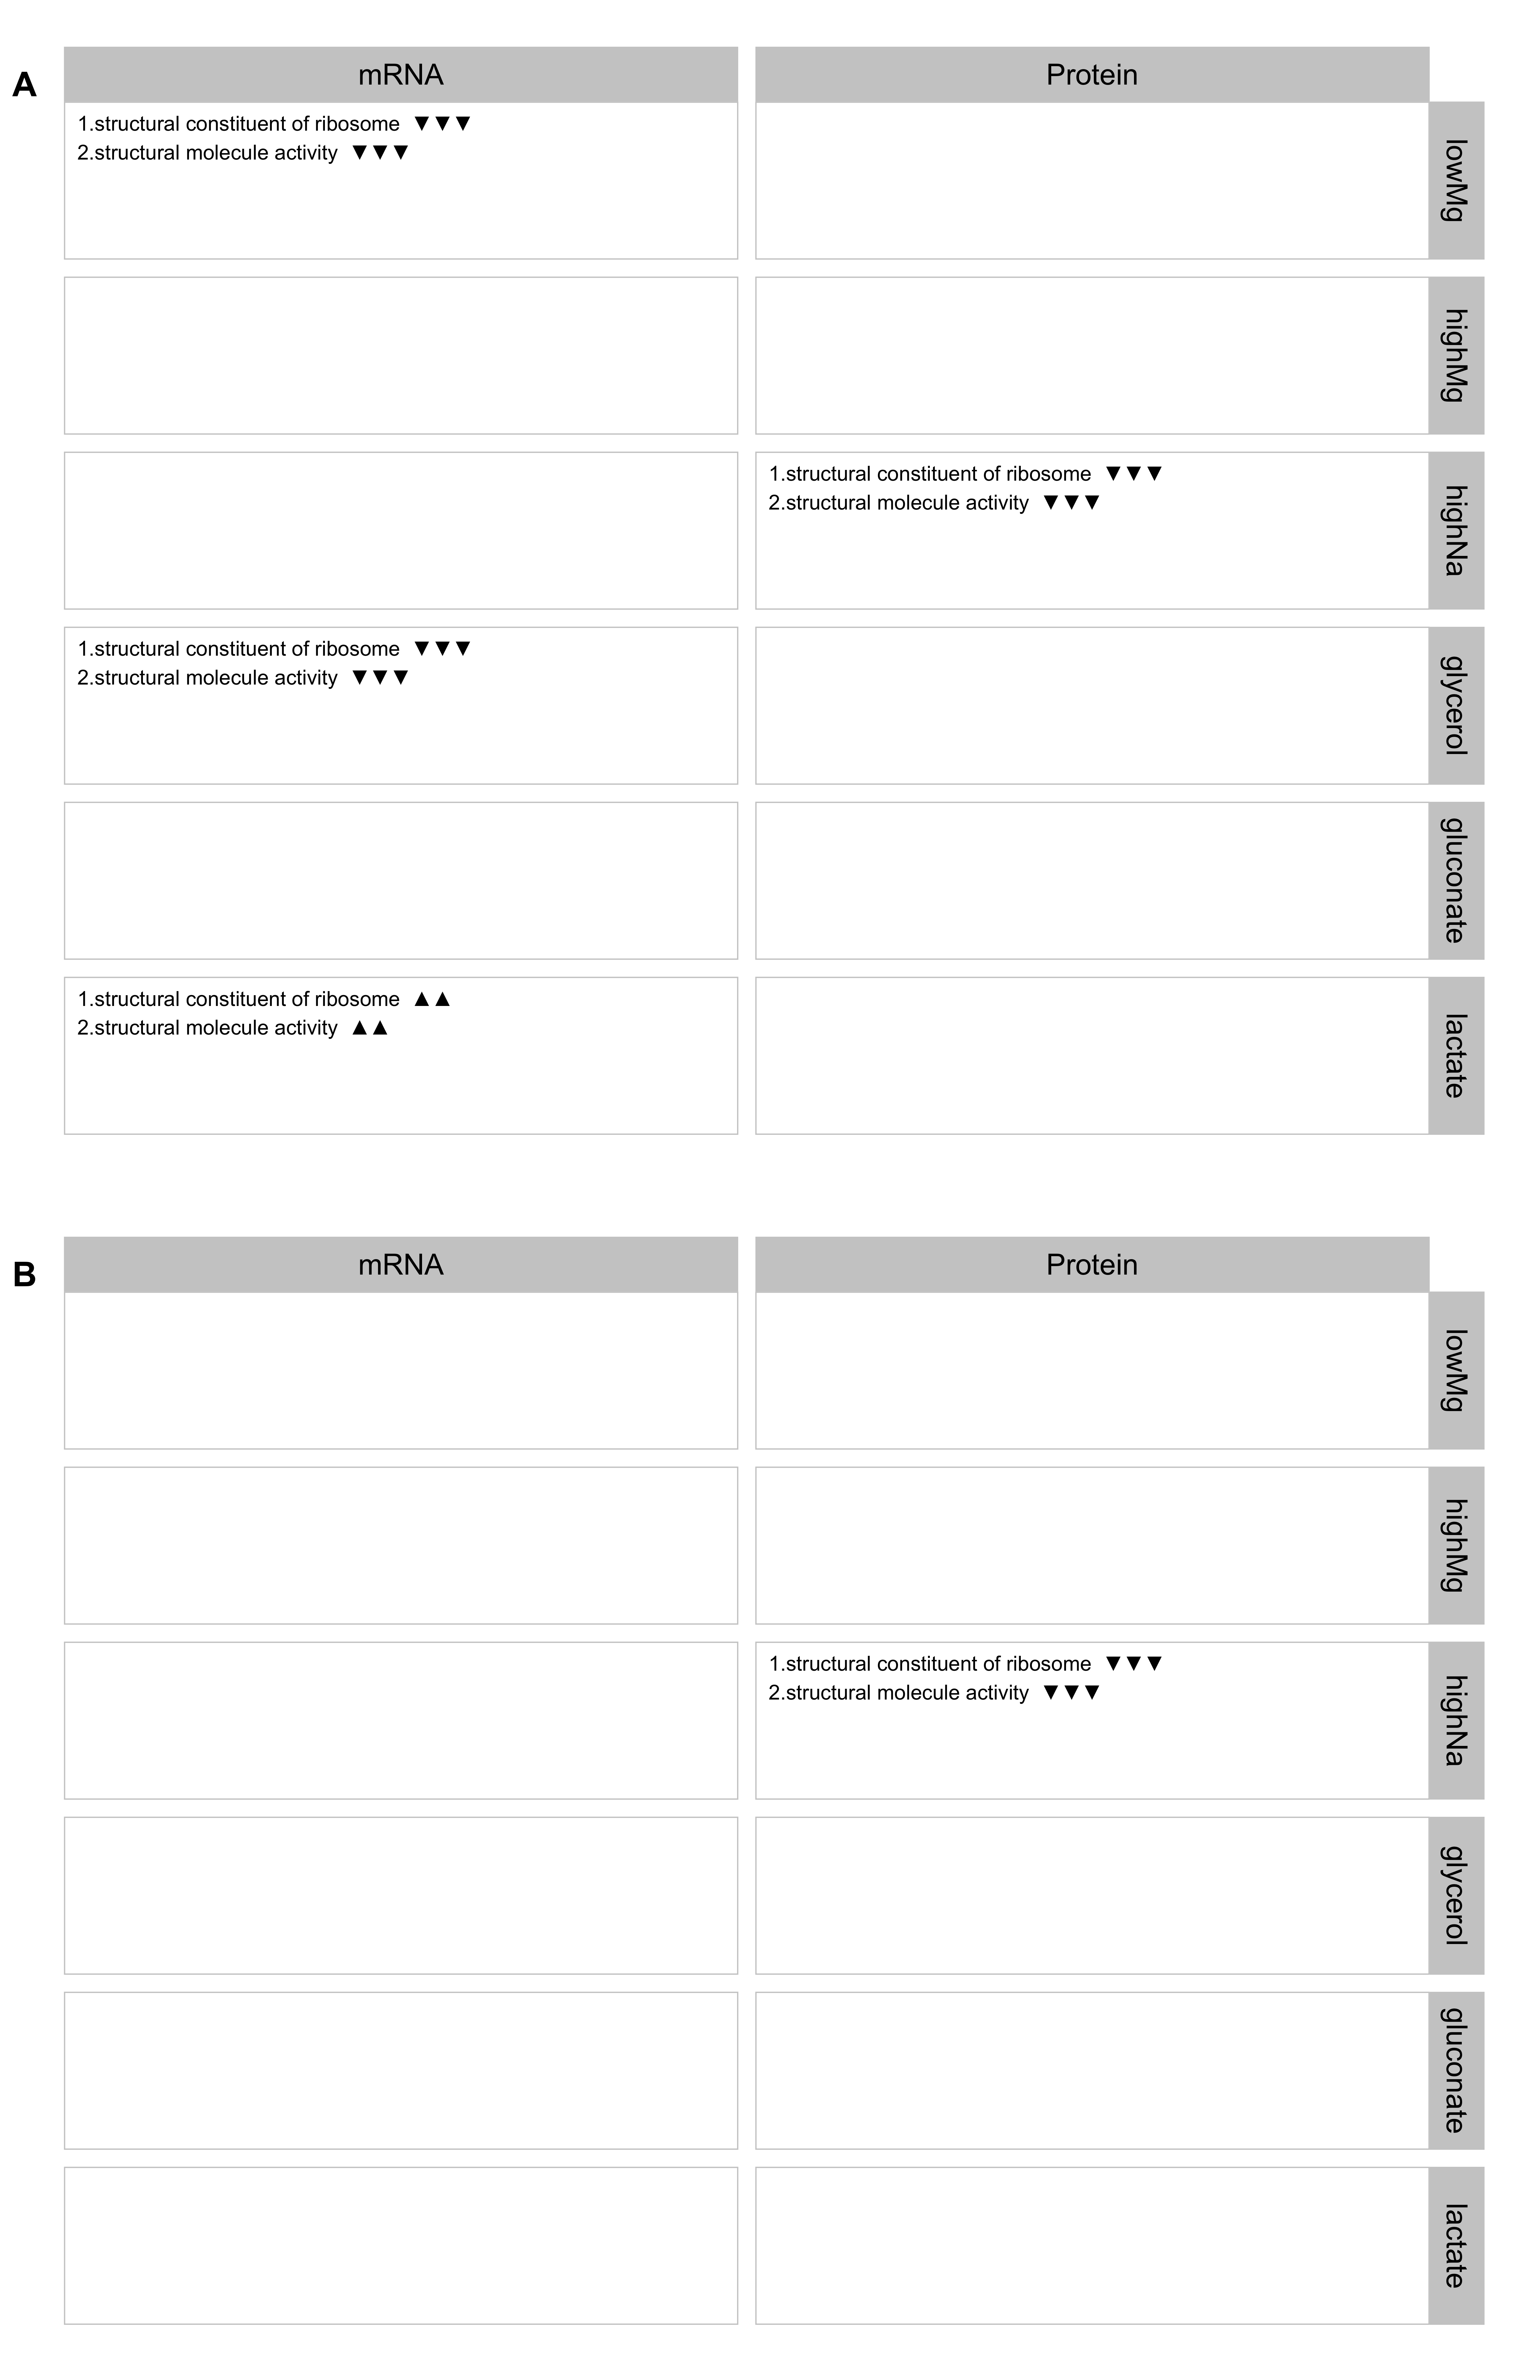
\includegraphics[width=0.7\textwidth]{../../d_figures/resultTable_mf.png}
}
	\caption[Significantly differentially expressed molecular functions]
	{\textbf{Significantly differentially expressed molecular functions, as determined by GO annotations.} For each condition, we show the top-5 differentially expressed molecular functions according to either mRNA or protein abundances.  Empty boxes indicate that no differentially expressed pathways were found. The arrows next to pathway names indicate the proportion of up- and down-regulated genes among the significantly differentially expressed genes in this pathway. One up arrow indicates that 60\% or more of the genes are up-regulated, two arrows correspond to 80\% or more genes, and three arrows correspond to 95\% or more genes being up-regulated. Similarly, down arrows indicate the proportion of down-regulated genes. (A) Exponential phase. (B) Stationary phase.}
\end{figure}

\clearpage

\begin{figure}[!htb]
	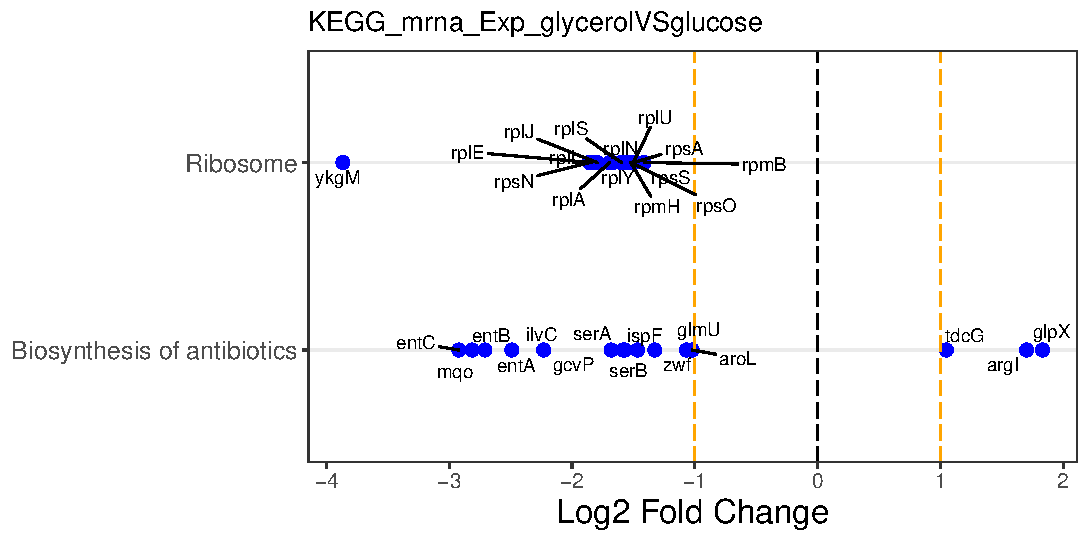
\includegraphics[width=1.0\textwidth]{../../d_figures/KEGG01_mrna_Exp_glycerolVSglucose_withTitle.pdf}
	\caption[Significantly differentially expressed KEGG pathways for mRNA samples in exponential phase tested for glycerol against glucose]
	{\textbf{Significantly differentially expressed KEGG pathways and associated genes with glycerol as carbon source, as determined by mRNA abundances in exponential phase.} The top 2 differentially expressed KEGG pathways are shown along the $y$ axis, and the relative fold change of the corresponding genes is shown along the $x$ axis. We show up to 10 of the most significantly changed pathways and for each pathway we show up to 15 of the most significantly changing genes.}
\end{figure}

\clearpage
\begin{figure}
	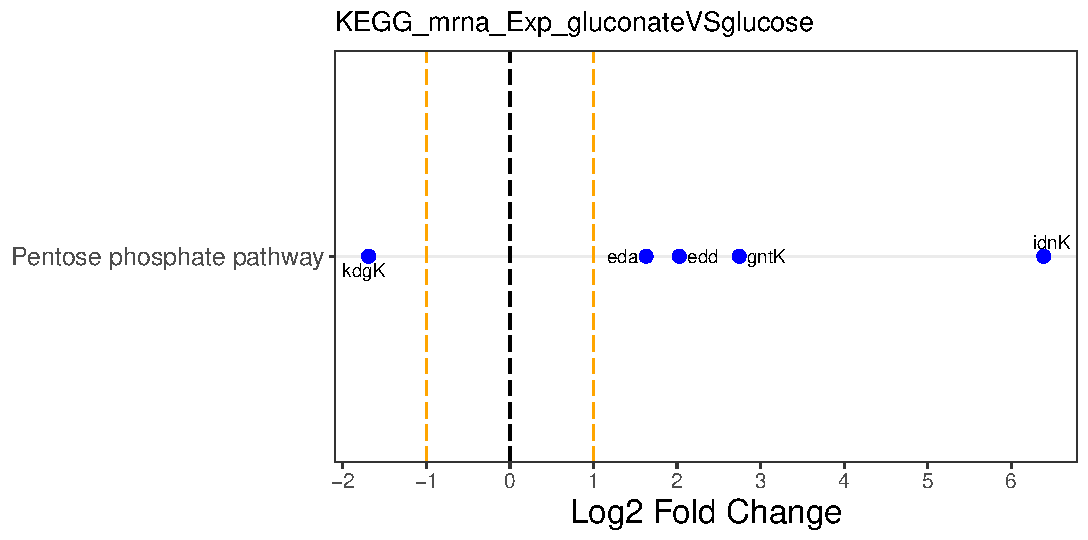
\includegraphics[width=1.0\textwidth]{../../d_figures/KEGG02_mrna_Exp_gluconateVSglucose_withTitle.pdf}
	\caption[Significantly differentially expressed KEGG pathways for mRNA samples in exponential phase tested for gluconate against glucose]
	{\textbf{Significantly differentially expressed KEGG pathway and associated genes with gluconate as carbon source, as determined by mRNA abundances in exponential phase.} The top differentially expressed KEGG pathway is shown along the $y$ axis, and the relative fold change of the corresponding genes is shown along the $x$ axis. We show up to 10 of the most significantly changed pathways and for each pathway we show up to 15 of the most significantly changing genes.}
\end{figure}

\clearpage
\begin{figure}
	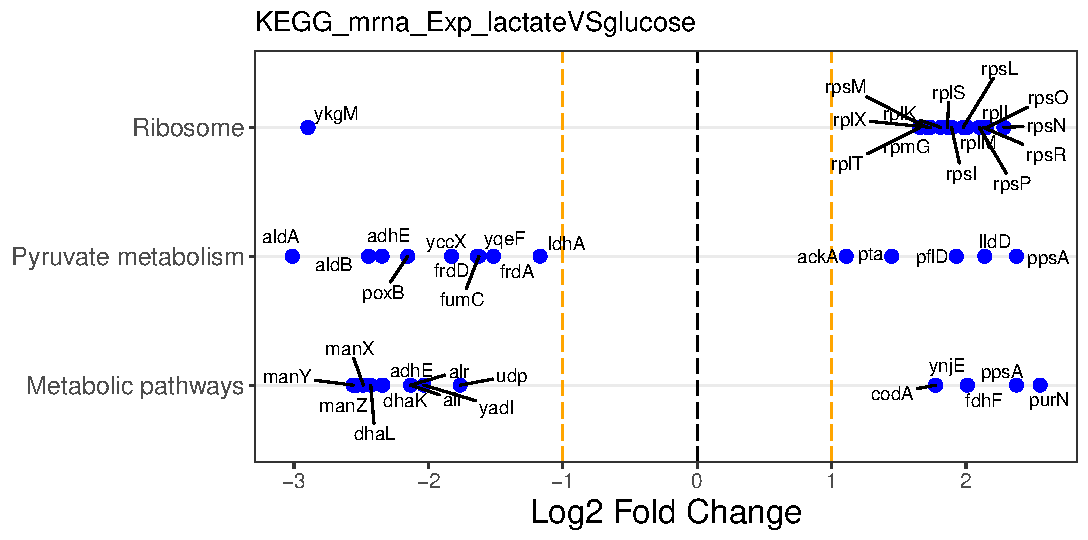
\includegraphics[width=1.0\textwidth]{../../d_figures/KEGG03_mrna_Exp_lactateVSglucose_withTitle.pdf}
	\caption[Significantly differentially expressed KEGG pathways for mRNA samples in exponential phase tested for lactate against glucose]
	{\textbf{Significantly differentially expressed KEGG pathways and associated genes with lactate as carbon source, as determined by mRNA abundances in exponential phase.} The top 3 differentially expressed KEGG pathways are shown along the $y$ axis, and the relative fold change of the corresponding genes is shown along the $x$ axis. We show up to 10 of the most significantly changed pathways and for each pathway we show up to 15 of the most significantly changing genes.}
\end{figure}

\clearpage
\begin{figure}
	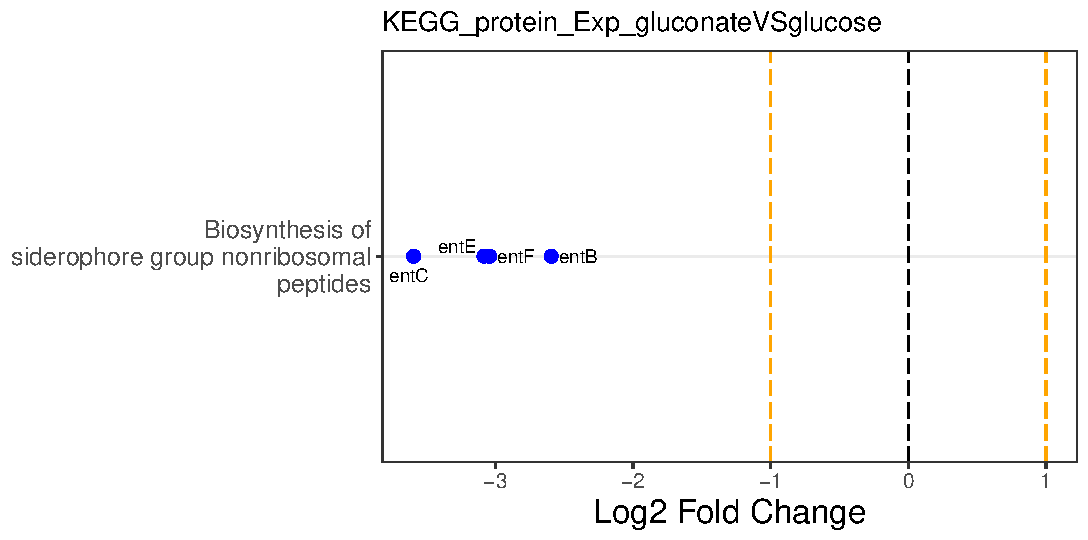
\includegraphics[width=1.0\textwidth]{../../d_figures/KEGG04_protein_Exp_gluconateVSglucose_withTitle.pdf}
	\caption[Significantly differentially expressed KEGG pathway for protein samples in exponential phase tested for gluconate against glucose]
	{\textbf{Significantly differentially expressed KEGG pathway and associated genes with gluconate as carbon source, as determined by protein abundances in exponential phase.} The top differentially expressed KEGG pathway is shown along the $y$ axis, and the relative fold change of the corresponding genes is shown along the $x$ axis. We show up to 10 of the most significantly changed pathways and for each pathway we show up to 15 of the most significantly changing genes.}
\end{figure}

\clearpage
\begin{figure}
	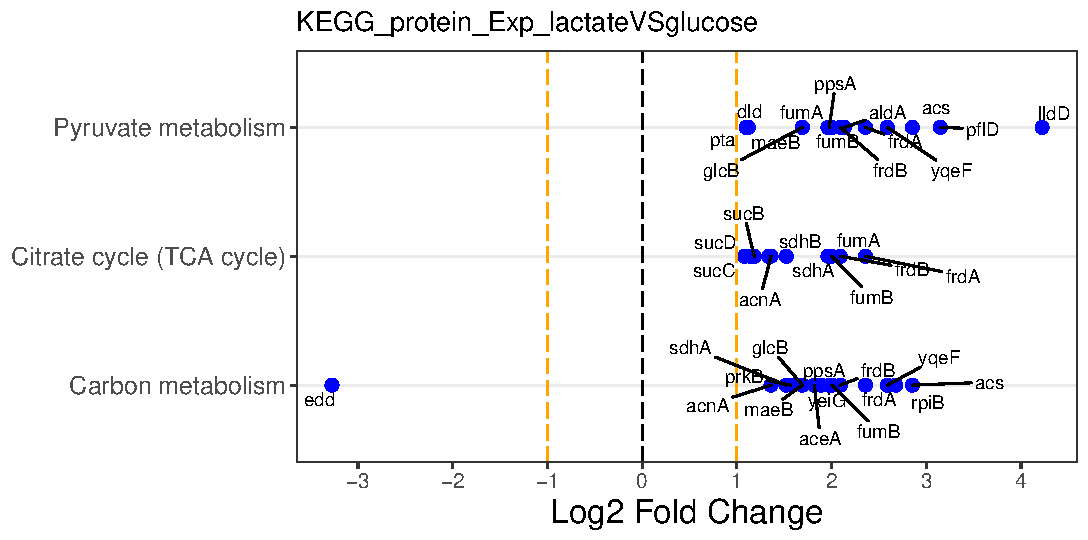
\includegraphics[width=1.0\textwidth]{../../d_figures/KEGG05_protein_Exp_lactateVSglucose_withTitle.pdf}
	\caption[Significantly differentially expressed KEGG pathways for protein samples in exponential phase tested for lactate against glucose]
	{\textbf{Significantly differentially expressed KEGG pathways and associated genes with lactate as carbon source, as determined by protein abundances in exponential phase.} The top 3 differentially expressed KEGG pathways are shown along the $y$ axis, and the relative fold change of the corresponding genes is shown along the $x$ axis. We show up to 10 of the most significantly changed pathways and for each pathway we show up to 15 of the most significantly changing genes.}
\end{figure}

\clearpage
\begin{figure}
	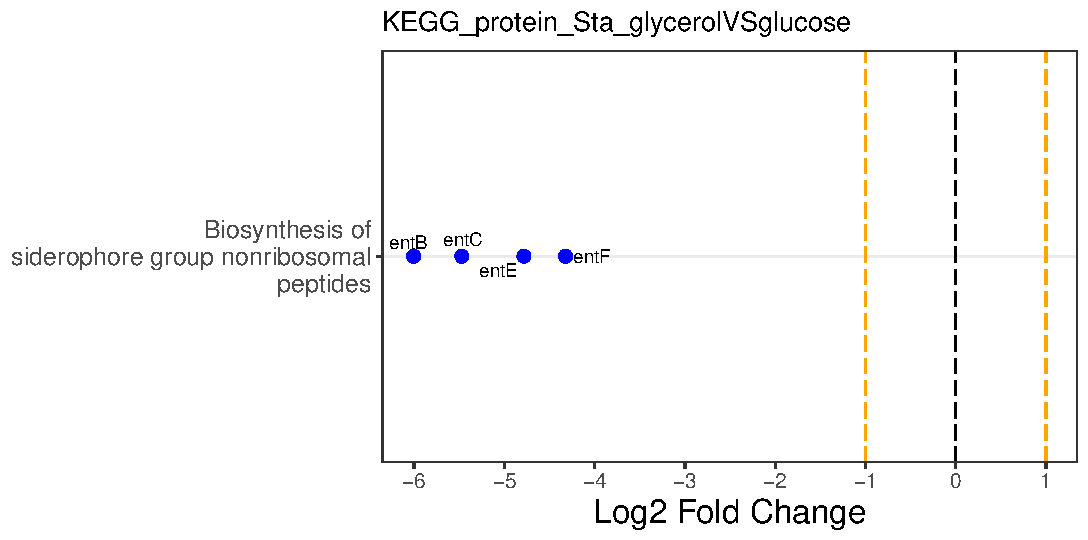
\includegraphics[width=1.0\textwidth]{../../d_figures/KEGG06_protein_Sta_glycerolVSglucose_withTitle.pdf}
	\caption[Significantly differentially expressed KEGG pathway for protein samples in stationary phase tested for glycerol against glucose]
	{\textbf{Significantly differentially expressed KEGG pathway and associated genes with glycerol as carbon source, as determined by protein abundances in stationary phase.} The top differentially expressed KEGG pathway is shown along the $y$ axis, and the relative fold change of the corresponding genes is shown along the $x$ axis. We show up to 10 of the most significantly changed pathways and for each pathway, we show up to 15 of the most significantly changing genes.}
\end{figure}

\clearpage
\begin{figure}
	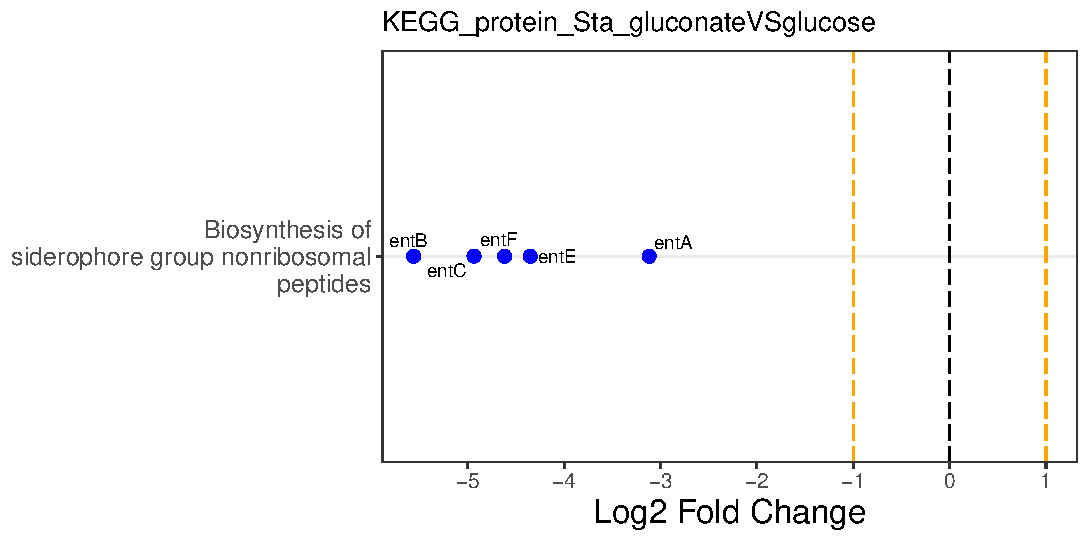
\includegraphics[width=1.0\textwidth]{../../d_figures/KEGG07_protein_Sta_gluconateVSglucose_withTitle.pdf}
	\caption[Significantly differentially expressed KEGG pathway for protein samples in stationary phase tested for gluconate against glucose]
	{\textbf{Significantly differentially expressed KEGG pathway and associated genes with gluconate as carbon source, as determined by protein abundances in stationary phase.} The top differentially expressed KEGG pathway is shown along the $y$ axis, and the relative fold change of the corresponding genes is shown along the $x$ axis. We show up to 10 of the most significantly changed pathways and for each pathway, we show up to 15 of the most significantly changing genes.}
\end{figure}

\clearpage
\begin{figure}
	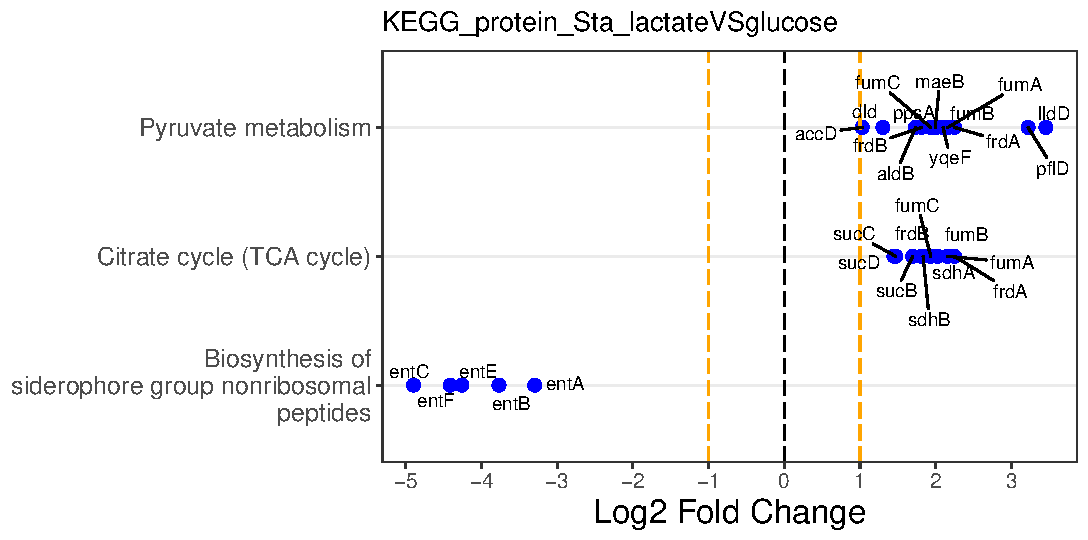
\includegraphics[width=1.0\textwidth]{../../d_figures/KEGG08_protein_Sta_lactateVSglucose_withTitle.pdf}
	\caption[Significantly differentially expressed KEGG pathways for protein samples in stationary phase tested for lactate against glucose]
	{\textbf{Significantly differentially expressed KEGG pathways and associated genes with lactate as carbon source, as determined by protein abundances in stationary phase.} The top 3 differentially expressed KEGG pathways are shown along the $y$ axis, and the relative fold change of the corresponding genes is shown along the $x$ axis. We show up to 10 of the most significantly changed pathways and for each pathway, we show up to 15 of the most significantly changing genes.}
\end{figure}

\clearpage
\begin{figure}
	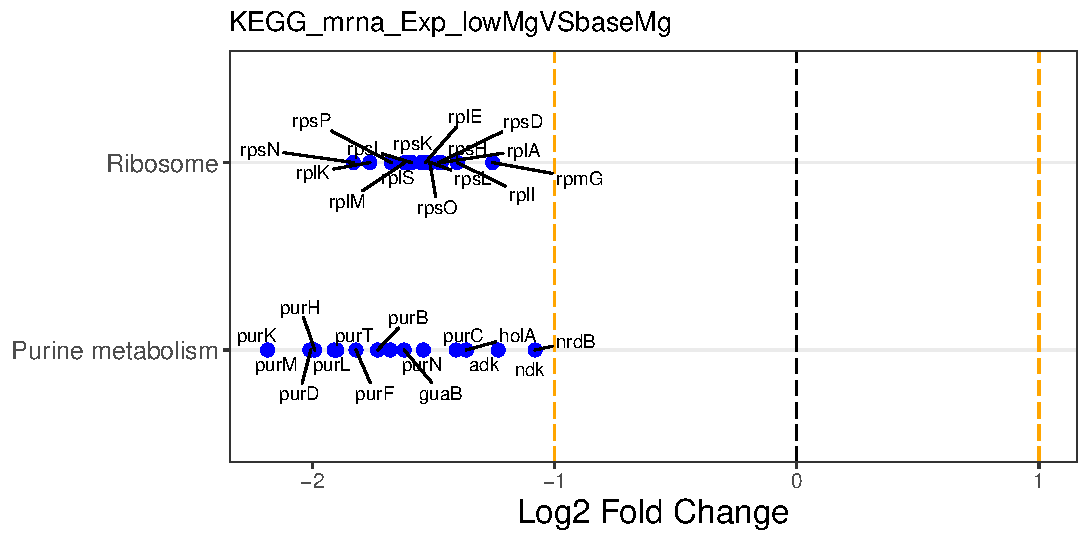
\includegraphics[width=1.0\textwidth]{../../d_figures/KEGG09_mrna_Exp_lowMgVSbaseMg_withTitle.pdf}
	\caption[Significantly differentially expressed KEGG pathways for mRNA samples in exponential phase tested for low Mg\textsuperscript{2+} levels against base Mg\textsuperscript{2+}]
	{\textbf{Significantly differentially expressed KEGG pathways and associated genes with low Mg\textsuperscript{2+} levels, as determined by mRNA abundances in exponential phase.} The top 2 differentially expressed KEGG pathways are shown along the $y$ axis, and the relative fold change of the corresponding genes is shown along the $x$ axis. We show up to 10 of the most significantly changed pathways and for each pathway, we show up to 15 of the most significantly changing genes.}
\end{figure}

\clearpage
\begin{figure}
	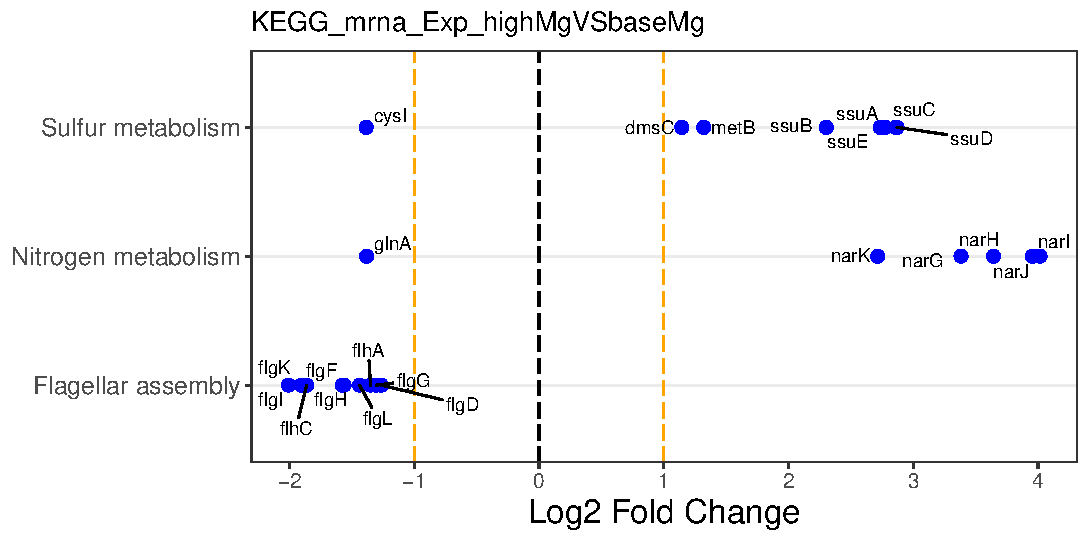
\includegraphics[width=1.0\textwidth]{../../d_figures/KEGG10_mrna_Exp_highMgVSbaseMg_withTitle.pdf}
	\caption[Significantly differentially expressed KEGG pathways for mRNA samples in exponential phase tested for high Mg\textsuperscript{2+} against base Mg\textsuperscript{2+}]
	{\textbf{Significantly differentially expressed KEGG pathways and associated genes with high Mg\textsuperscript{2+} levels, as determined by mRNA abundances in exponential phase.} The top 3 differentially expressed KEGG pathways are shown along the $y$ axis, and the relative fold change of the corresponding genes is shown along the $x$ axis. We show up to 10 of the most significantly changed pathways and for each pathway, we show up to 15 of the most significantly changing genes.}
\end{figure}

\clearpage
\begin{figure}
	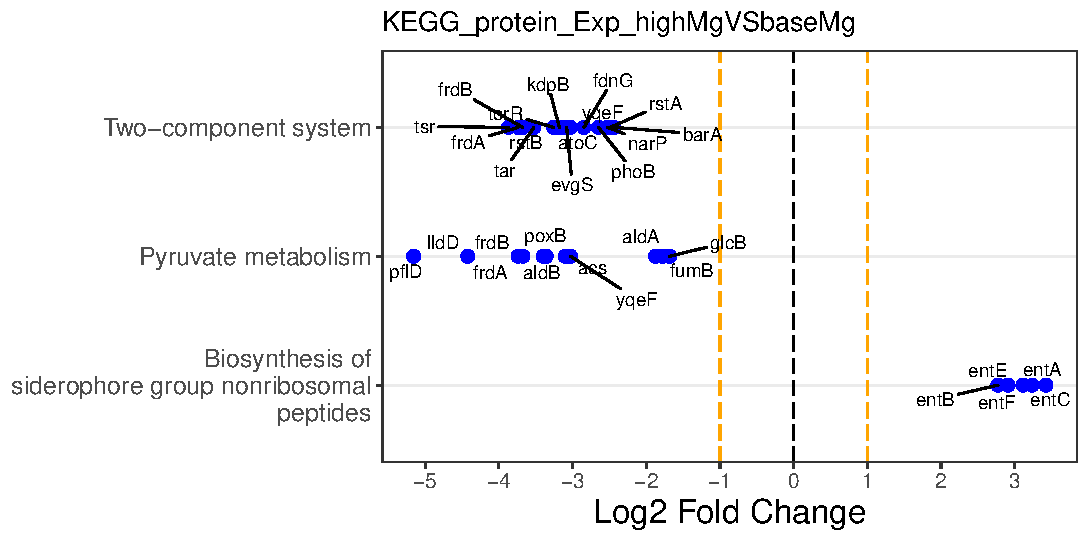
\includegraphics[width=1.0\textwidth]{../../d_figures/KEGG11_protein_Exp_highMgVSbaseMg_withTitle.pdf}
	\caption[Significantly differentially expressed KEGG pathways for protein samples in exponential phase tested for high Mg\textsuperscript{2+} against base Mg\textsuperscript{2+}]
	{\textbf{Significantly differentially expressed KEGG pathways and associated genes with high Mg\textsuperscript{2+} levels, as determined by protein abundances in exponential phase.} The top 3 differentially expressed KEGG pathways are shown along the $y$ axis, and the relative fold change of the corresponding genes is shown along the $x$ axis. We show up to 10 of the most significantly changed pathways and for each pathway, we show up to 15 of the most significantly changing genes.}
\end{figure}

\clearpage
\begin{figure}
	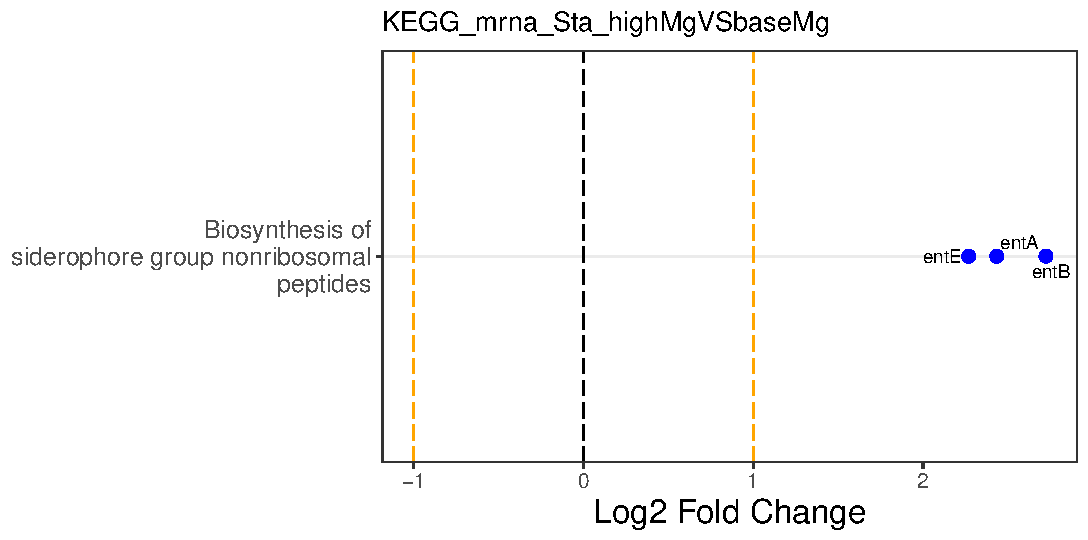
\includegraphics[width=1.0\textwidth]{../../d_figures/KEGG12_mrna_Sta_highMgVSbaseMg_withTitle.pdf}
	\caption[Significantly differentially expressed KEGG pathway for mRNA samples in stationary phase tested for high Mg\textsuperscript{2+} against base Mg\textsuperscript{2+}]
	{\textbf{Significantly differentially expressed KEGG pathway and associated genes with high Mg\textsuperscript{2+} levels, as determined by mRNA abundances in stationary phase.} The top differentially expressed KEGG pathway is shown along the $y$ axis, and the relative fold change of the corresponding genes is shown along the $x$ axis. We show up to 10 of the most significantly changed pathways and for each pathway, we show up to 15 of the most significantly changing genes.}
\end{figure}

\clearpage
\begin{figure}
	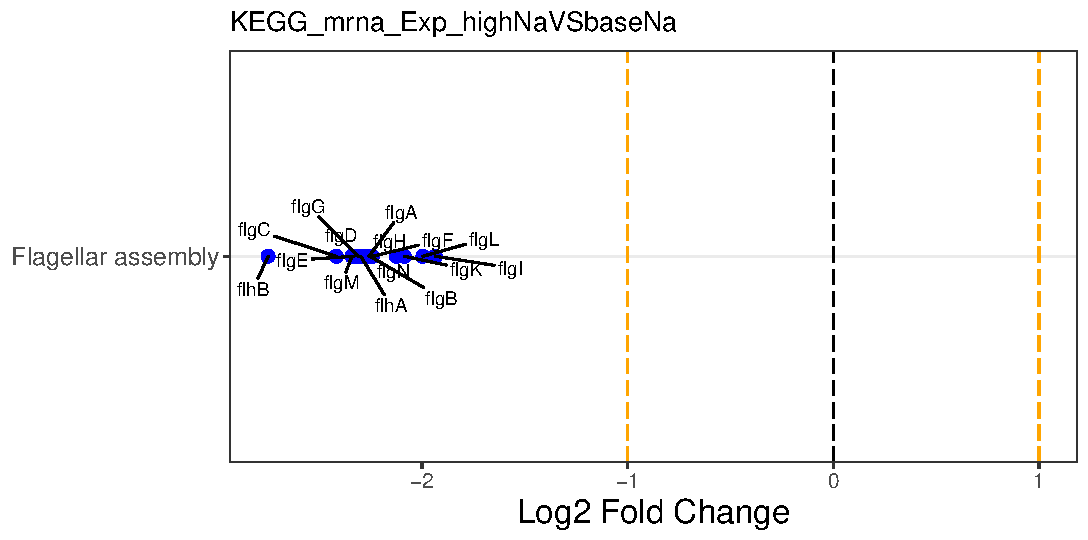
\includegraphics[width=1.0\textwidth]{../../d_figures/KEGG13_mrna_Exp_highNaVSbaseNa_withTitle.pdf}
	\caption[Significantly differentially expressed KEGG pathway for mRNA samples in exponential phase tested for high Na\textsuperscript{+} against base Na\textsuperscript{+}]
	{\textbf{Significantly differentially expressed KEGG pathway and associated genes with high Na\textsuperscript{+} levels, as determined by mRNA abundances in exponential phase.} The top differentially expressed KEGG pathway is shown along the $y$ axis, and the relative fold change of the corresponding genes is shown along the $x$ axis. We show up to 10 of the most significantly changed pathways and for each pathway, we show up to 15 of the most significantly changing genes.}
\end{figure}

\clearpage
\begin{figure}
	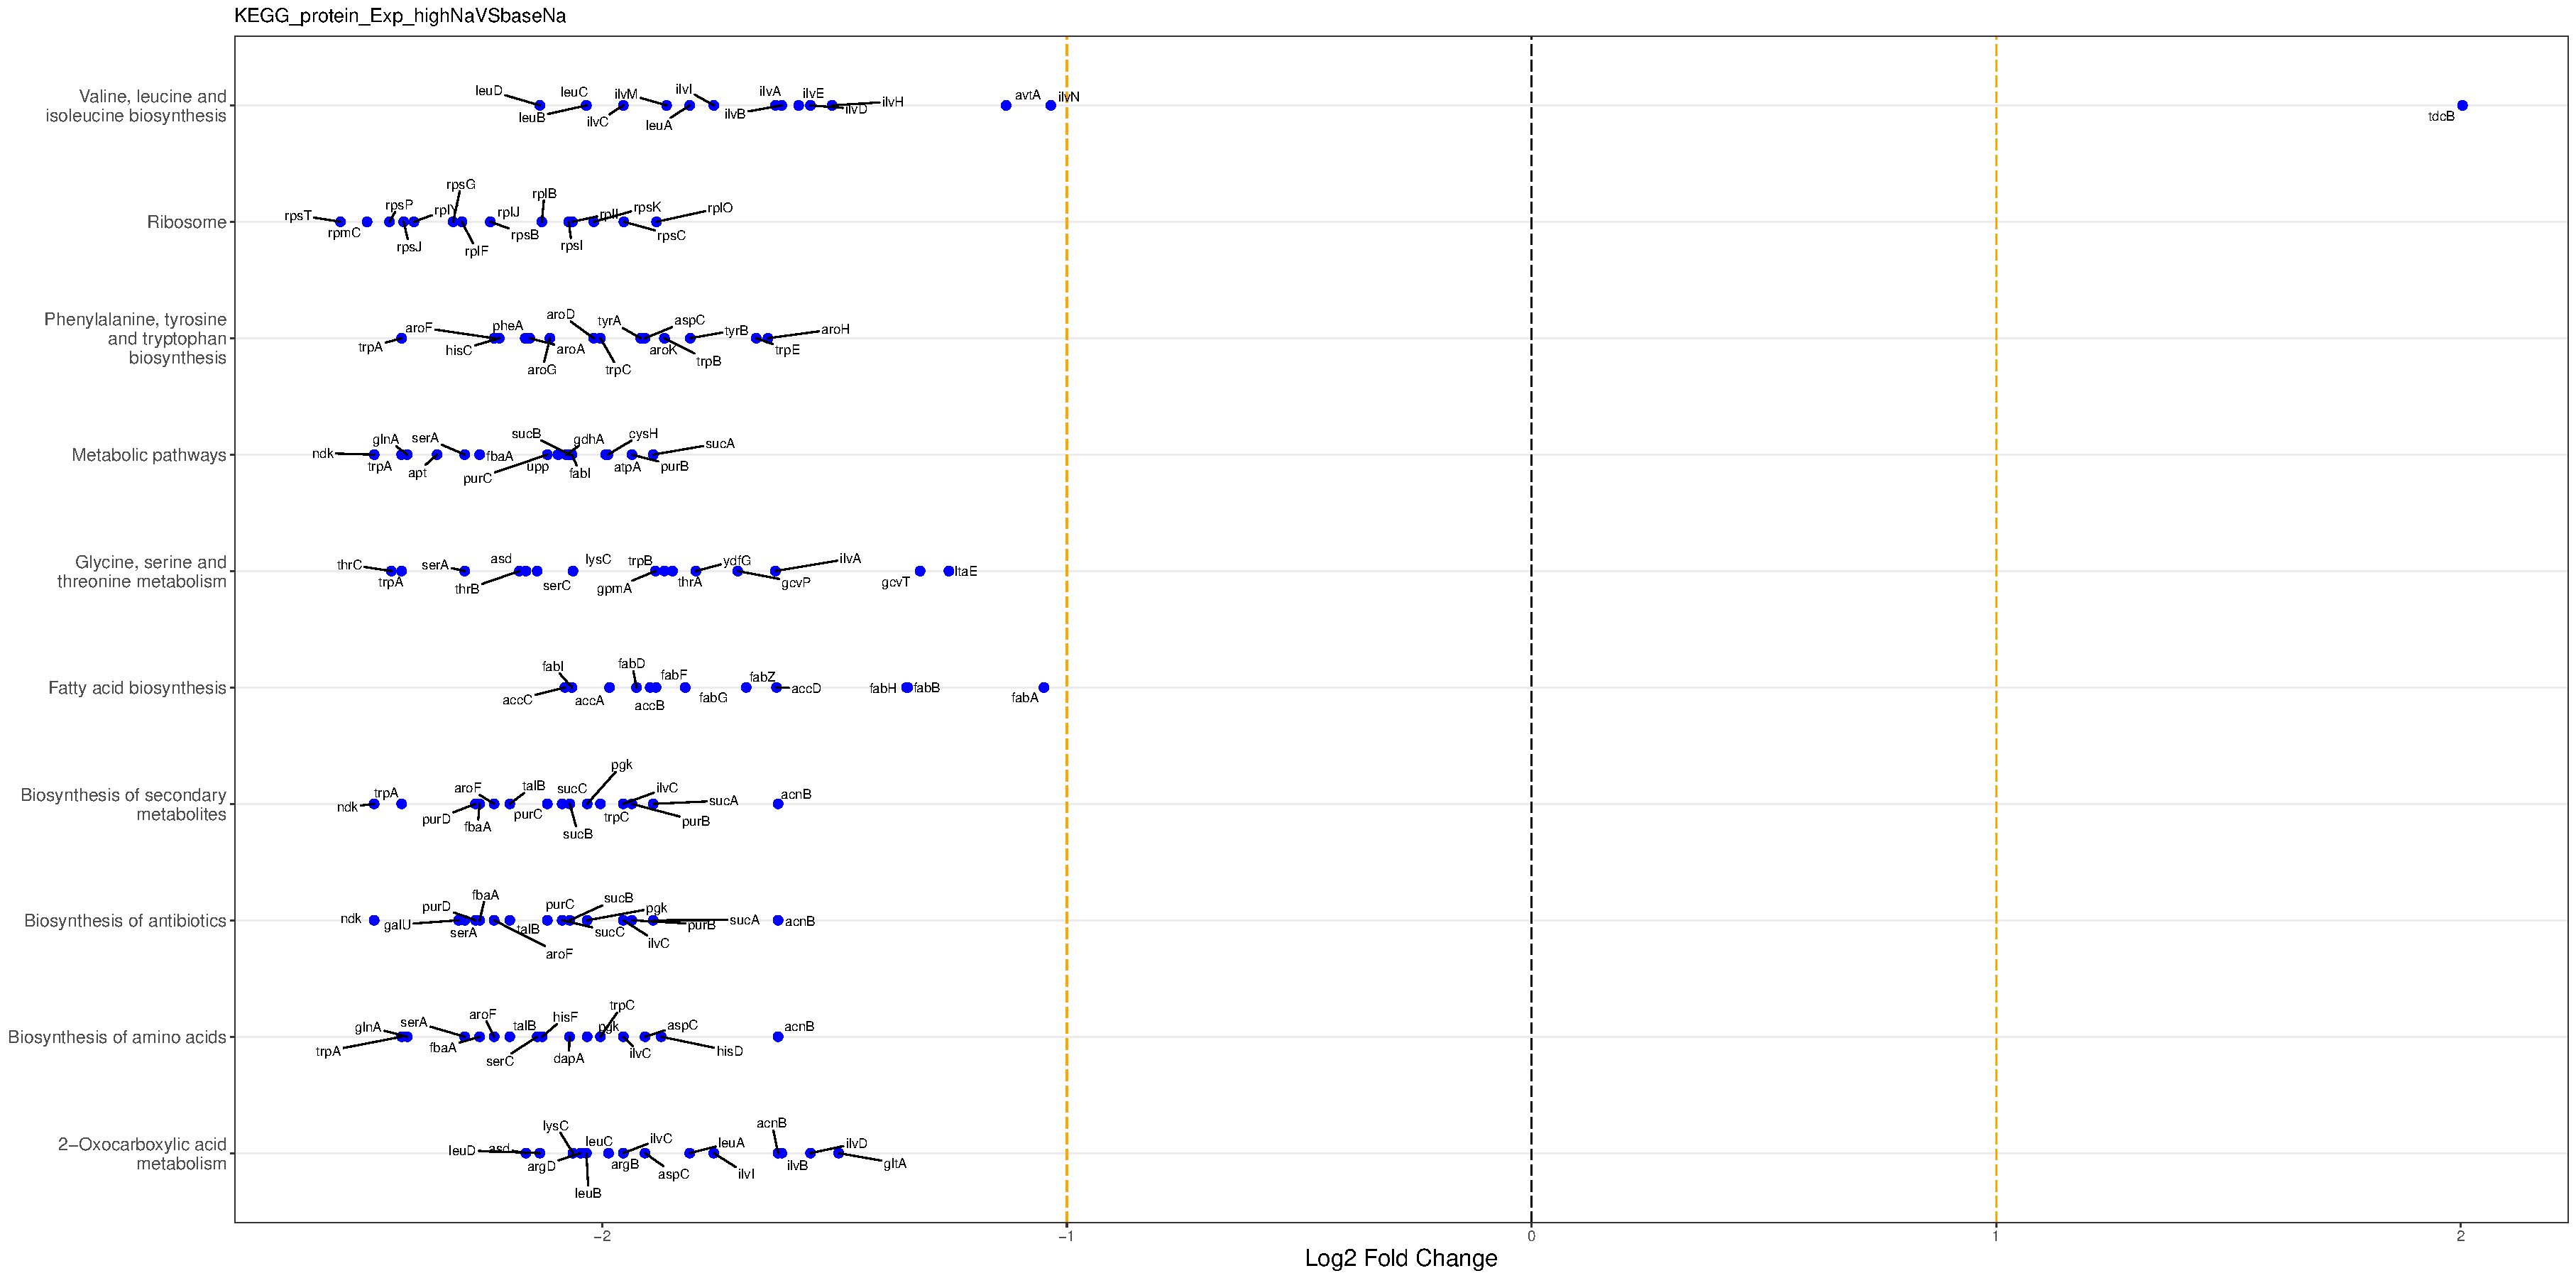
\includegraphics[width=1.0\textwidth]{../../d_figures/KEGG14_protein_Exp_highNaVSbaseNa_withTitle.pdf}
	\caption[Significantly differentially expressed KEGG pathways for protein samples in exponential phase tested for high Na\textsuperscript{+} against base Na\textsuperscript{+}]
	{\textbf{Significantly differentially expressed KEGG pathways and associated genes with high Na\textsuperscript{+} levels, as determined by protein abundances in exponential phase.} The top 10 differentially expressed KEGG pathways are shown along the $y$ axis, and the relative fold change of the corresponding genes is shown along the $x$ axis. We show up to 10 of the most significantly changed pathways and for each pathway, we show up to 15 of the most significantly changing genes.}
\end{figure}

\clearpage
\begin{figure}
	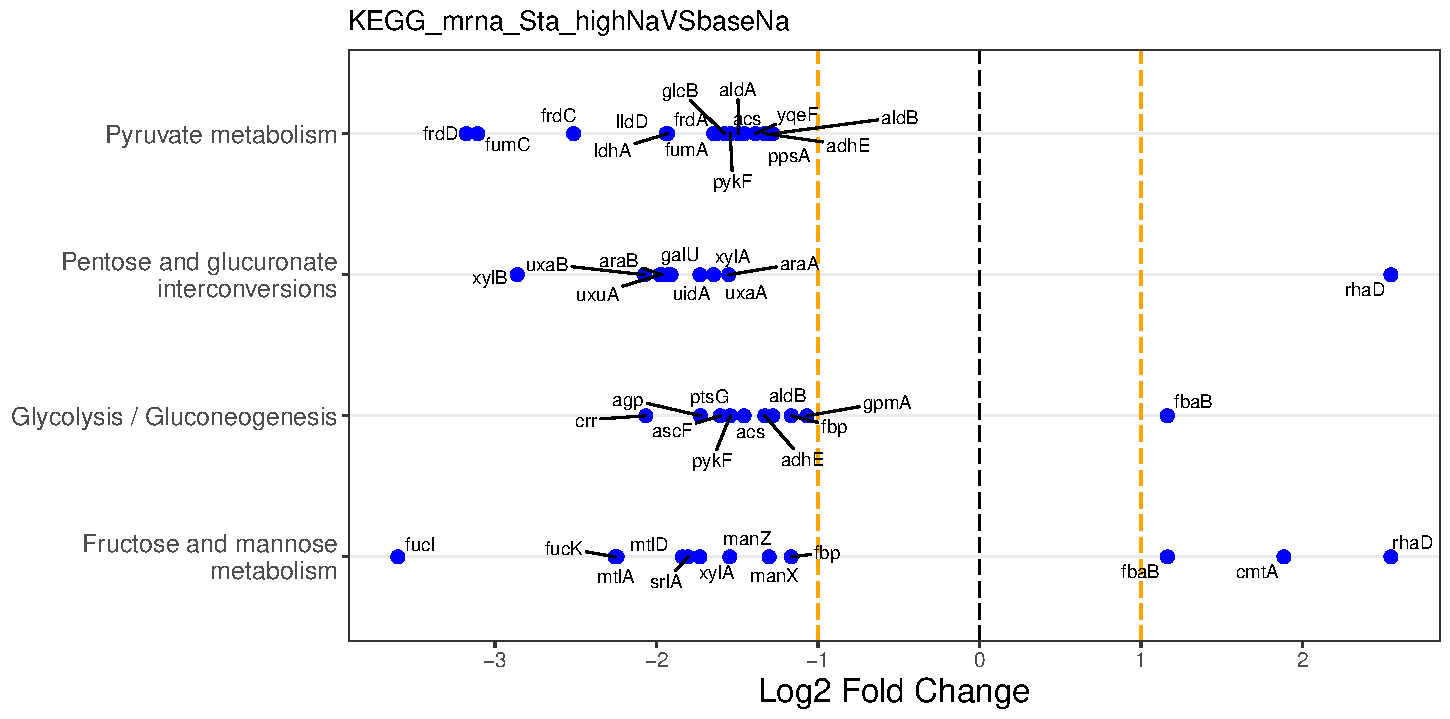
\includegraphics[width=1.0\textwidth]{../../d_figures/KEGG15_mrna_Sta_highNaVSbaseNa_withTitle.pdf}
	\caption[Significantly differentially expressed KEGG pathways for mRNA samples in stationary phase tested for high Na\textsuperscript{+} against base Na\textsuperscript{+}]
	{\textbf{Significantly differentially expressed KEGG pathways and associated genes with high Na\textsuperscript{+} levels, as determined by mRNA abundances in stationary phase.} The top 4 differentially expressed KEGG pathways are shown along the $y$ axis, and the relative fold change of the corresponding genes is shown along the $x$ axis. We show up to 10 of the most significantly changed pathways and for each pathway, we show up to 15 of the most significantly changing genes.}
\end{figure}

\clearpage
\begin{figure}
	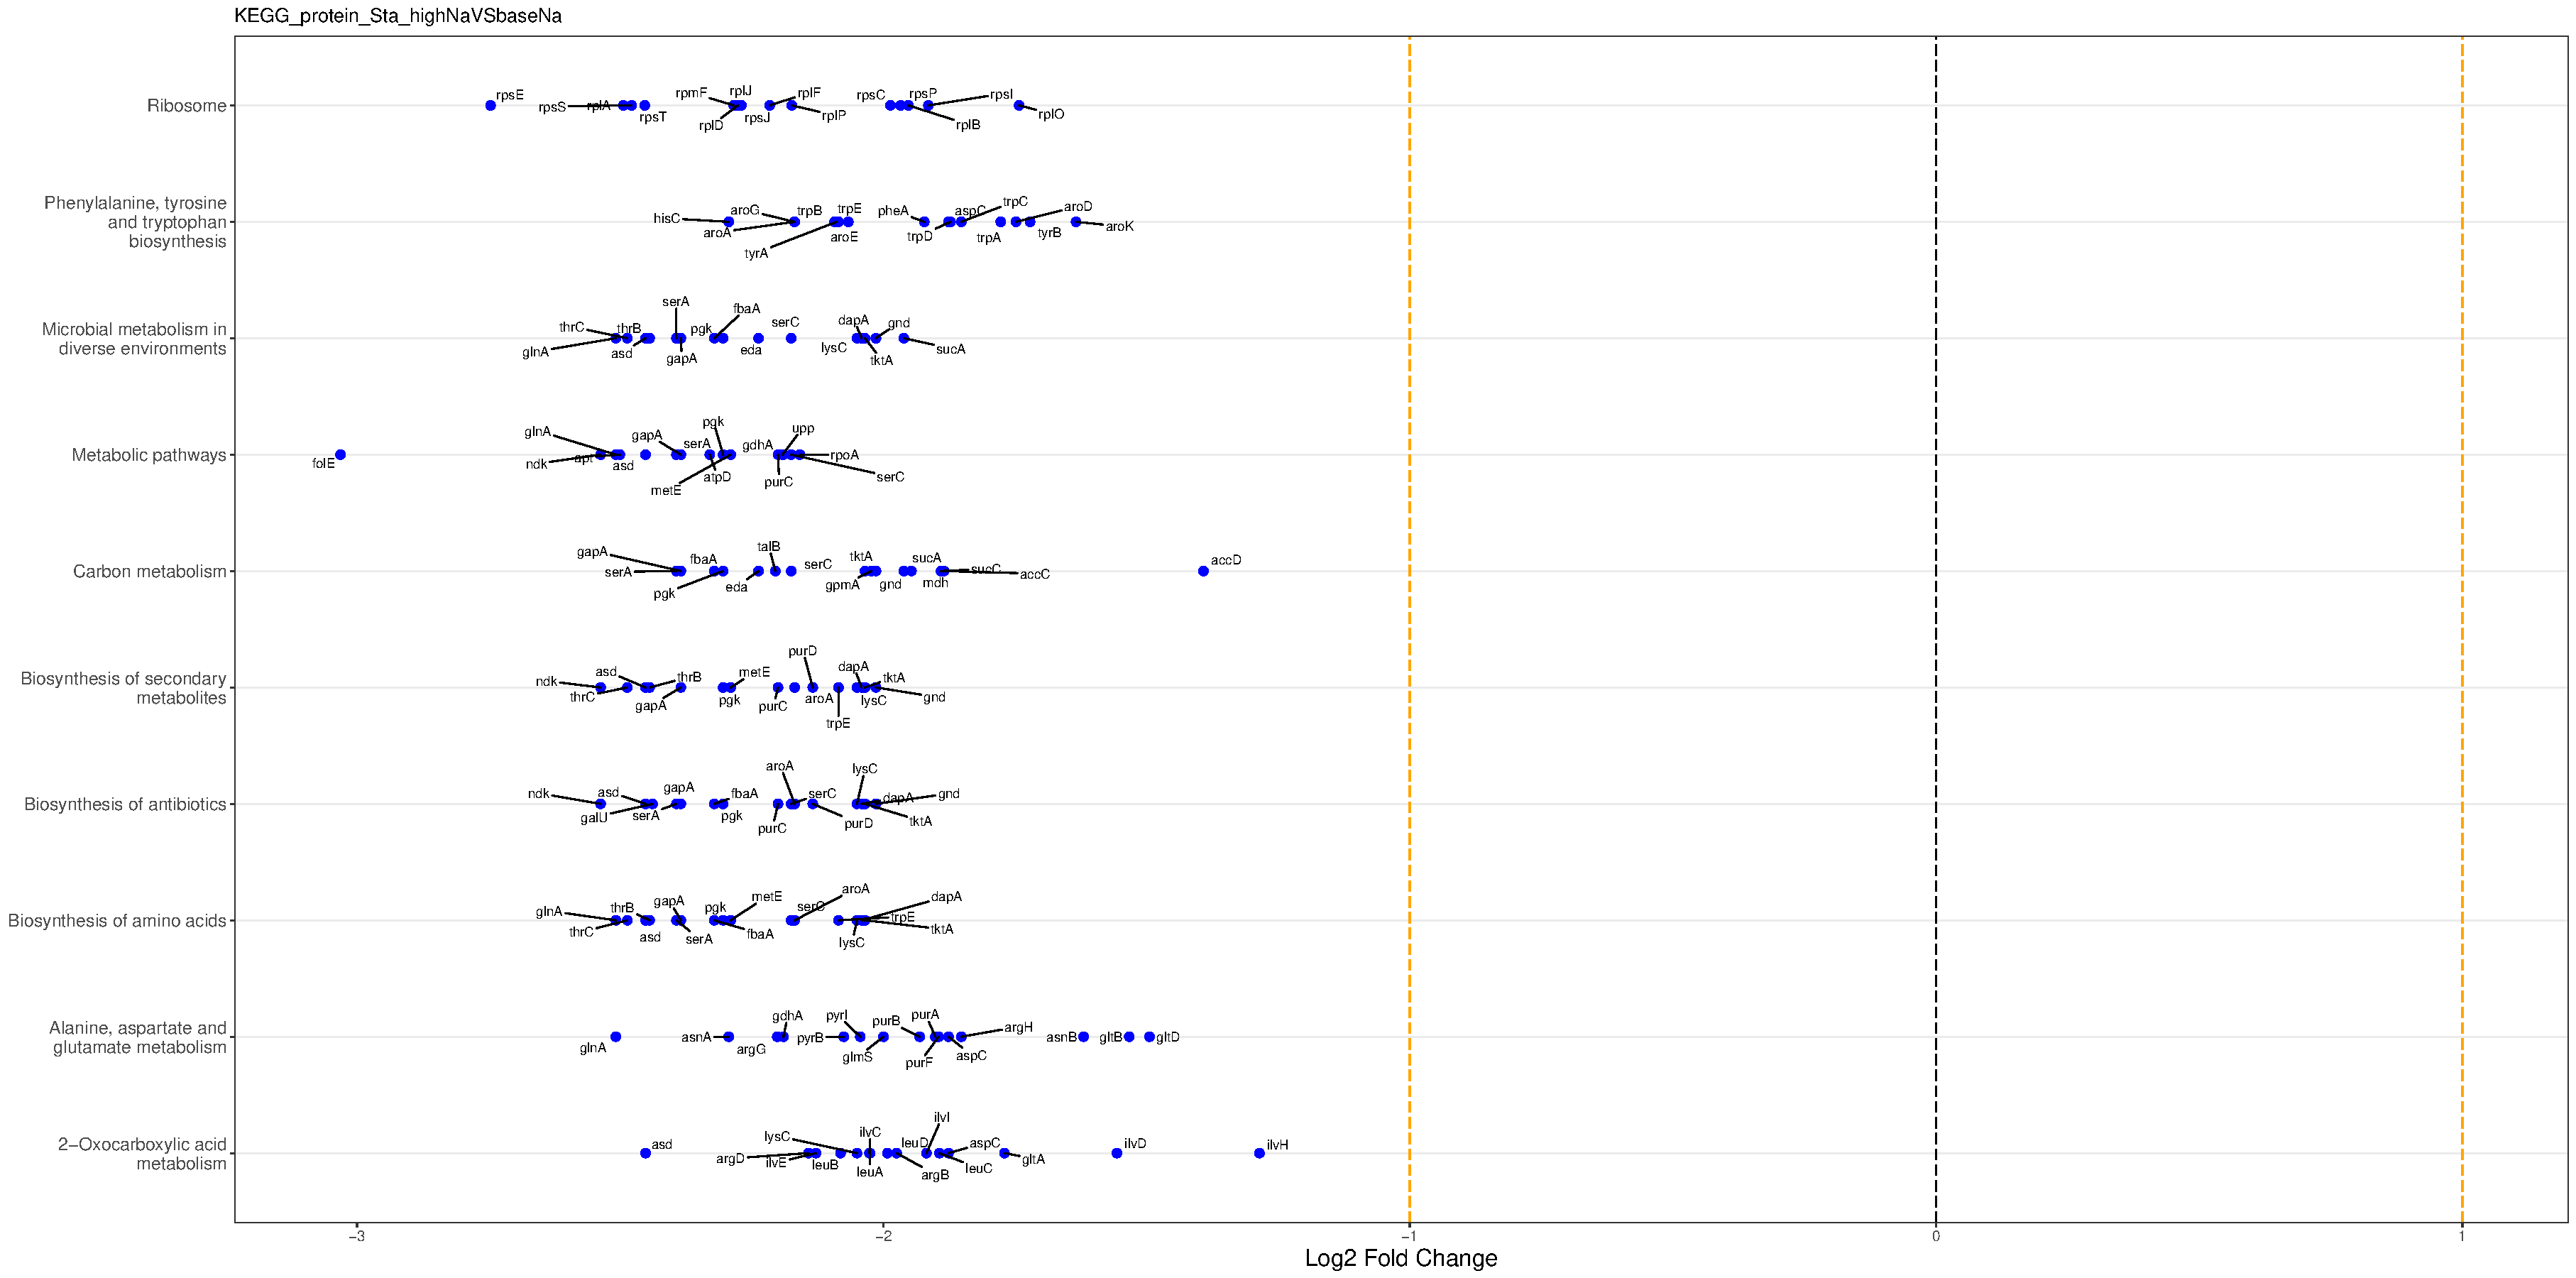
\includegraphics[width=1.0\textwidth]{../../d_figures/KEGG16_protein_Sta_highNaVSbaseNa_withTitle}
	\caption[Significantly differentially expressed KEGG pathways for protein samples in stationary phase tested for high Na\textsuperscript{+} against base Na\textsuperscript{+}]
	{\textbf{Significantly differentially expressed KEGG pathways and associated genes with high Na\textsuperscript{+} levels, as determined by protein abundances in stationary phase.} The top 10 differentially expressed KEGG pathways are shown along the $y$ axis, and the relative fold change of the corresponding genes is shown along the $x$ axis. We show up to 10 of the most significantly changed pathways and for each pathway, we show up to 15 of the most significantly changing genes.}
\end{figure}
\clearpage


\begin{figure}[!htb]
	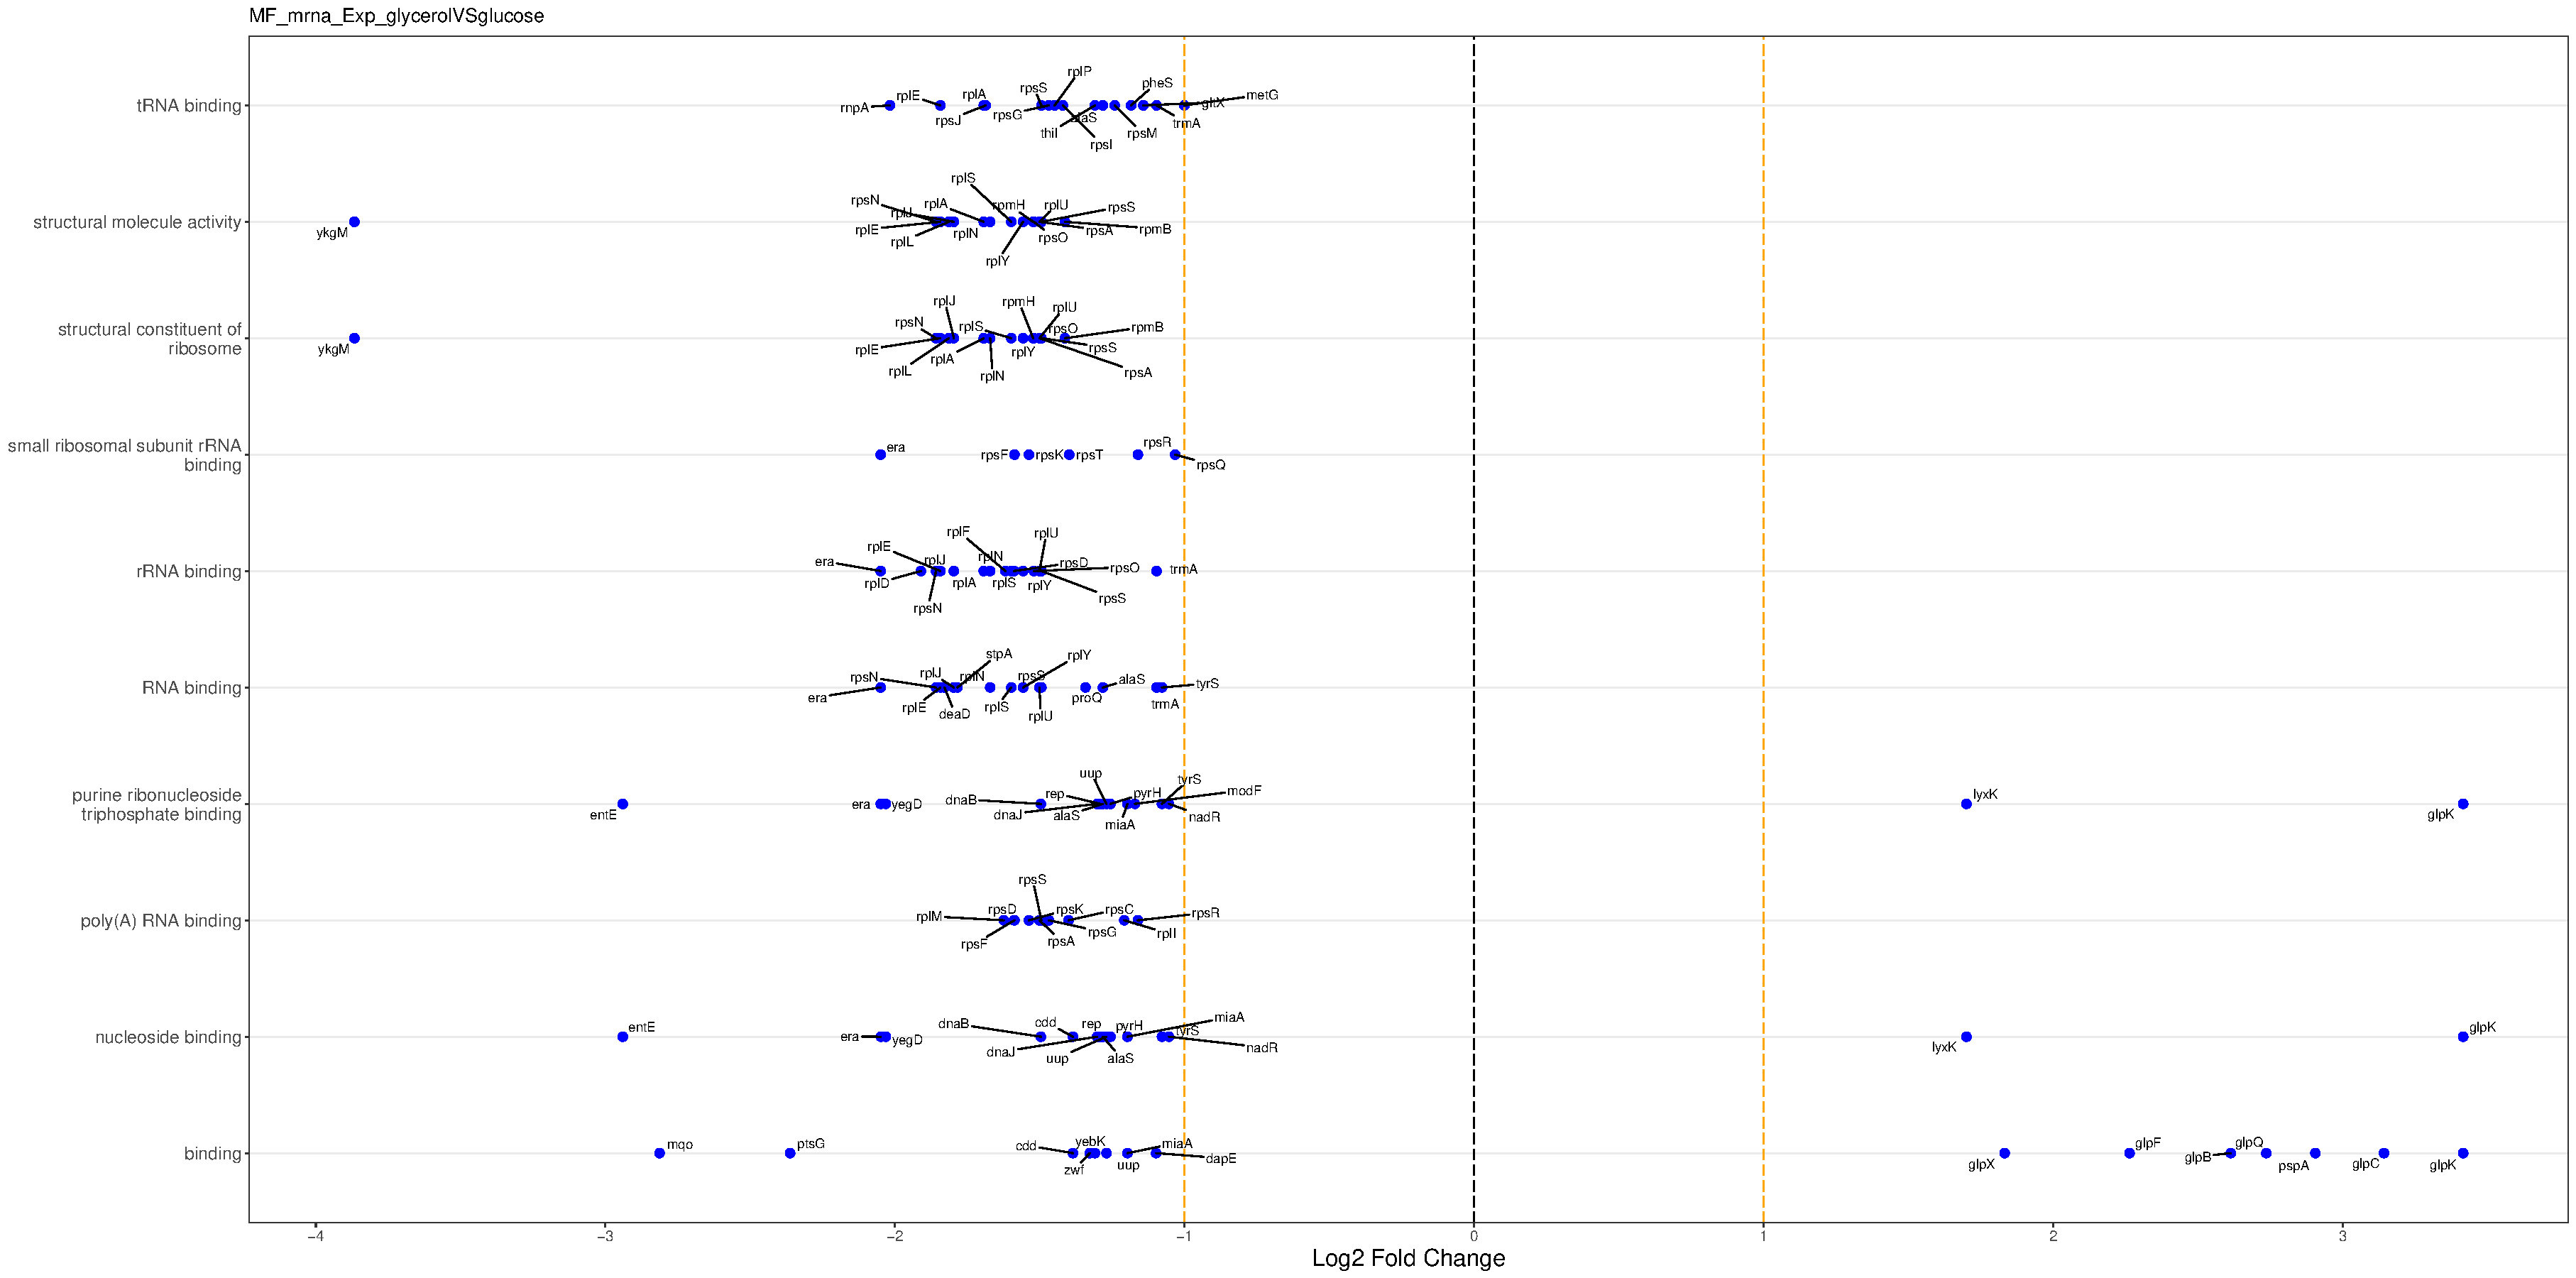
\includegraphics[width=1.0\textwidth]{../../d_figures/MF01_mrna_Exp_glycerolVSglucose_withTitle.pdf}
	\caption[Significantly differentially expressed GO annotations associated with molecular functions for mRNA samples in exponential phase tested for glycerol against glucose]
	{\textbf{Significantly differentially expressed GO annotations related with molecular functions and associated genes with glycerol as carbon source, as determined by mRNA abundances in exponential phase.} The top 10 differentially expressed molecular functions are shown along the $y$ axis, and the relative fold change of the corresponding genes is shown along the $x$ axis. We show up to 10 of the most significantly changed molecular functions and for each molecular function, we show up to 15 of the most significantly changing genes.}
\end{figure}


\begin{figure}[!htb]
	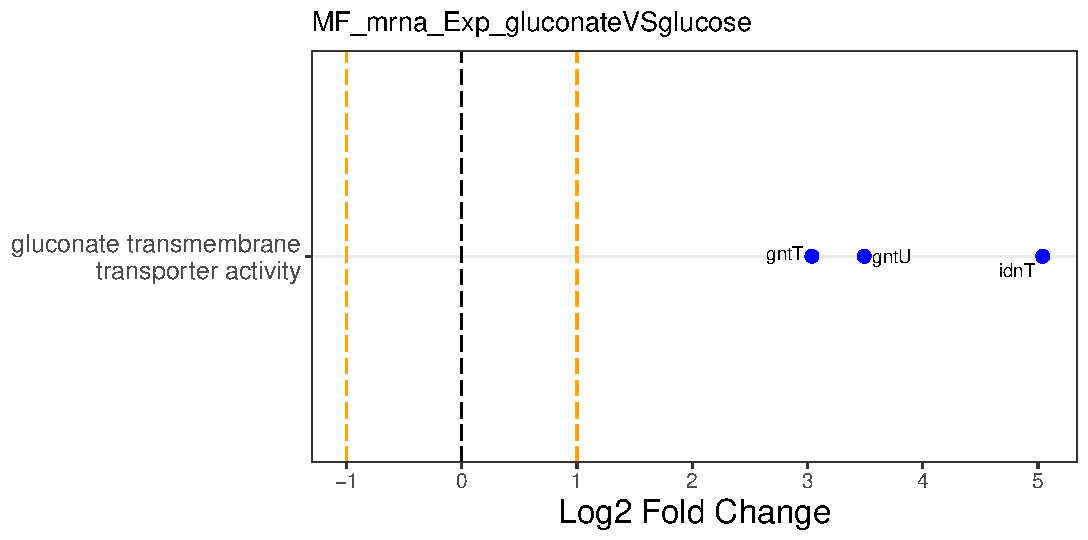
\includegraphics[width=1.0\textwidth]{../../d_figures/MF02_mrna_Exp_gluconateVSglucose_withTitle.pdf}
	\caption[Significantly differentially expressed GO annotations associated with molecular functions for mRNA samples in exponential phase tested for gluconate against glucose]
	{\textbf{Significantly differentially expressed GO annotations related with molecular functions and associated genes with gluconate as carbon source, as determined by mRNA abundances in exponential phase.} The top 2 differentially expressed molecular functions are shown along the $y$ axis, and the relative fold change of the corresponding genes is shown along the $x$ axis. We show up to 10 of the most significantly changed molecular functions and for each molecular function, we show up to 15 of the most significantly changing genes.}
\end{figure}

\begin{figure}[!htb]
	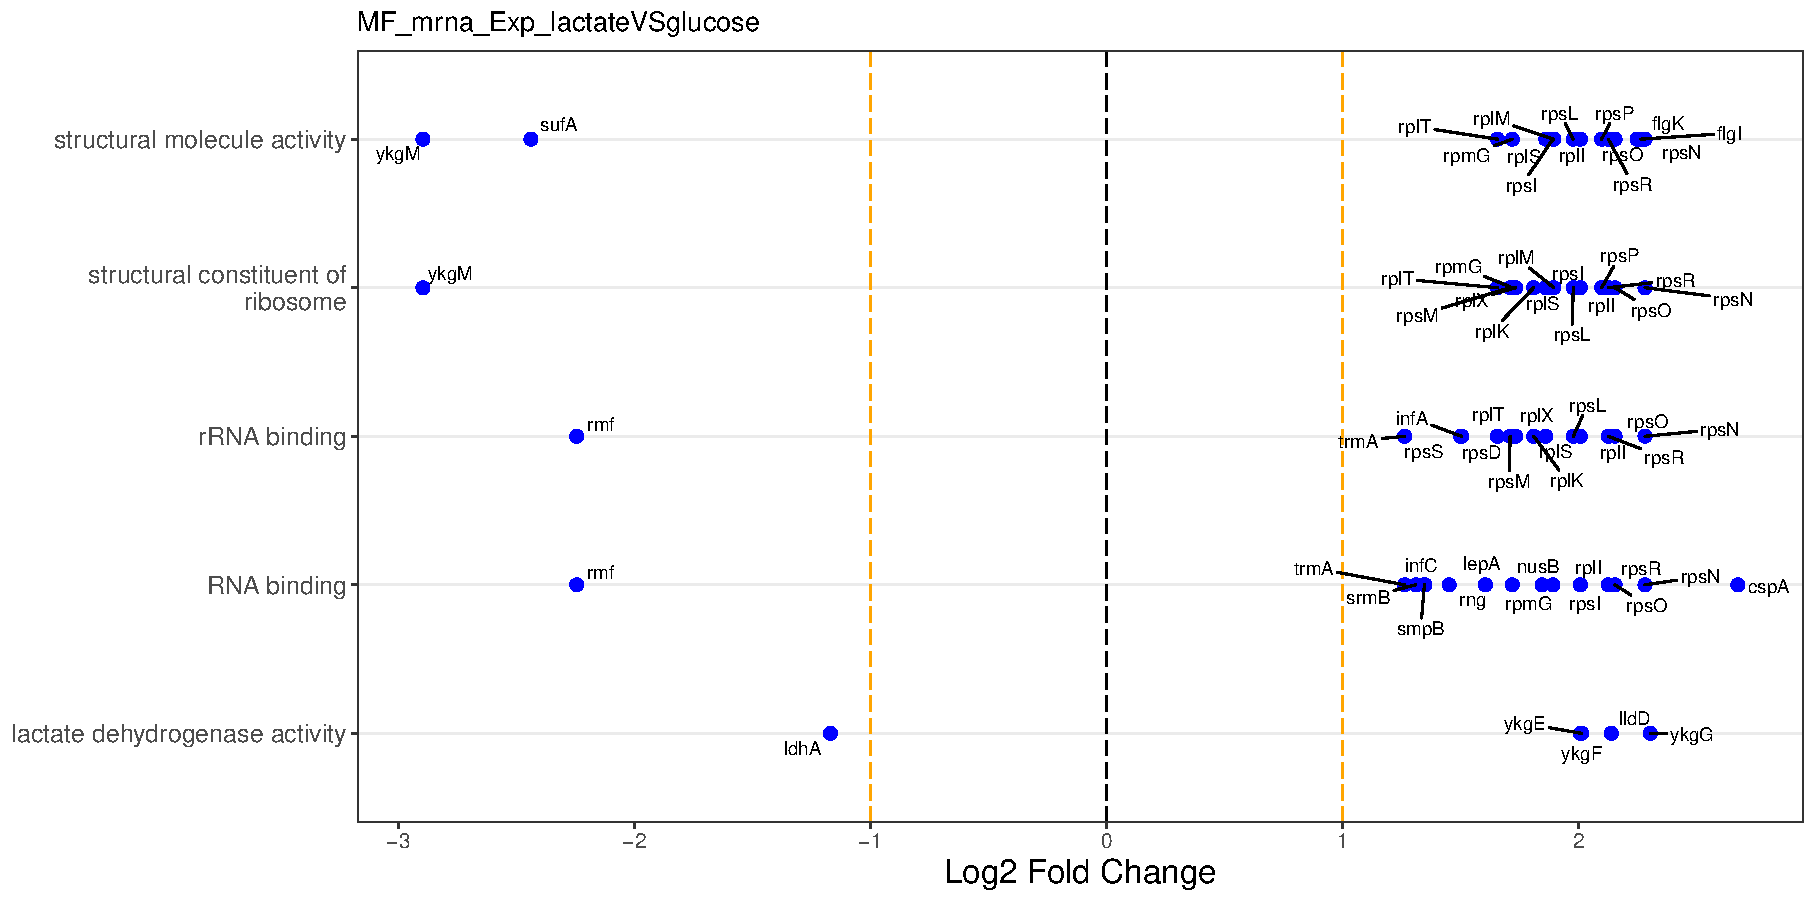
\includegraphics[width=1.0\textwidth]{../../d_figures/MF03_mrna_Exp_lactateVSglucose_withTitle.pdf}
	\caption[Significantly differentially expressed GO annotations associated with molecular functions for mRNA samples in exponential phase tested for lactate against glucose]
	{\textbf{Significantly differentially expressed GO annotations related with molecular functions and associated genes with lactate as carbon source, as determined by mRNA abundances in exponential phase.} The top 5 differentially expressed molecular functions are shown along the $y$ axis, and the relative fold change of the corresponding genes is shown along the $x$ axis. We show up to 10 of the most significantly changed molecular functions and for each molecular function, we show up to 15 of the most significantly changing genes.}
\end{figure}


\begin{figure}[!htb]
	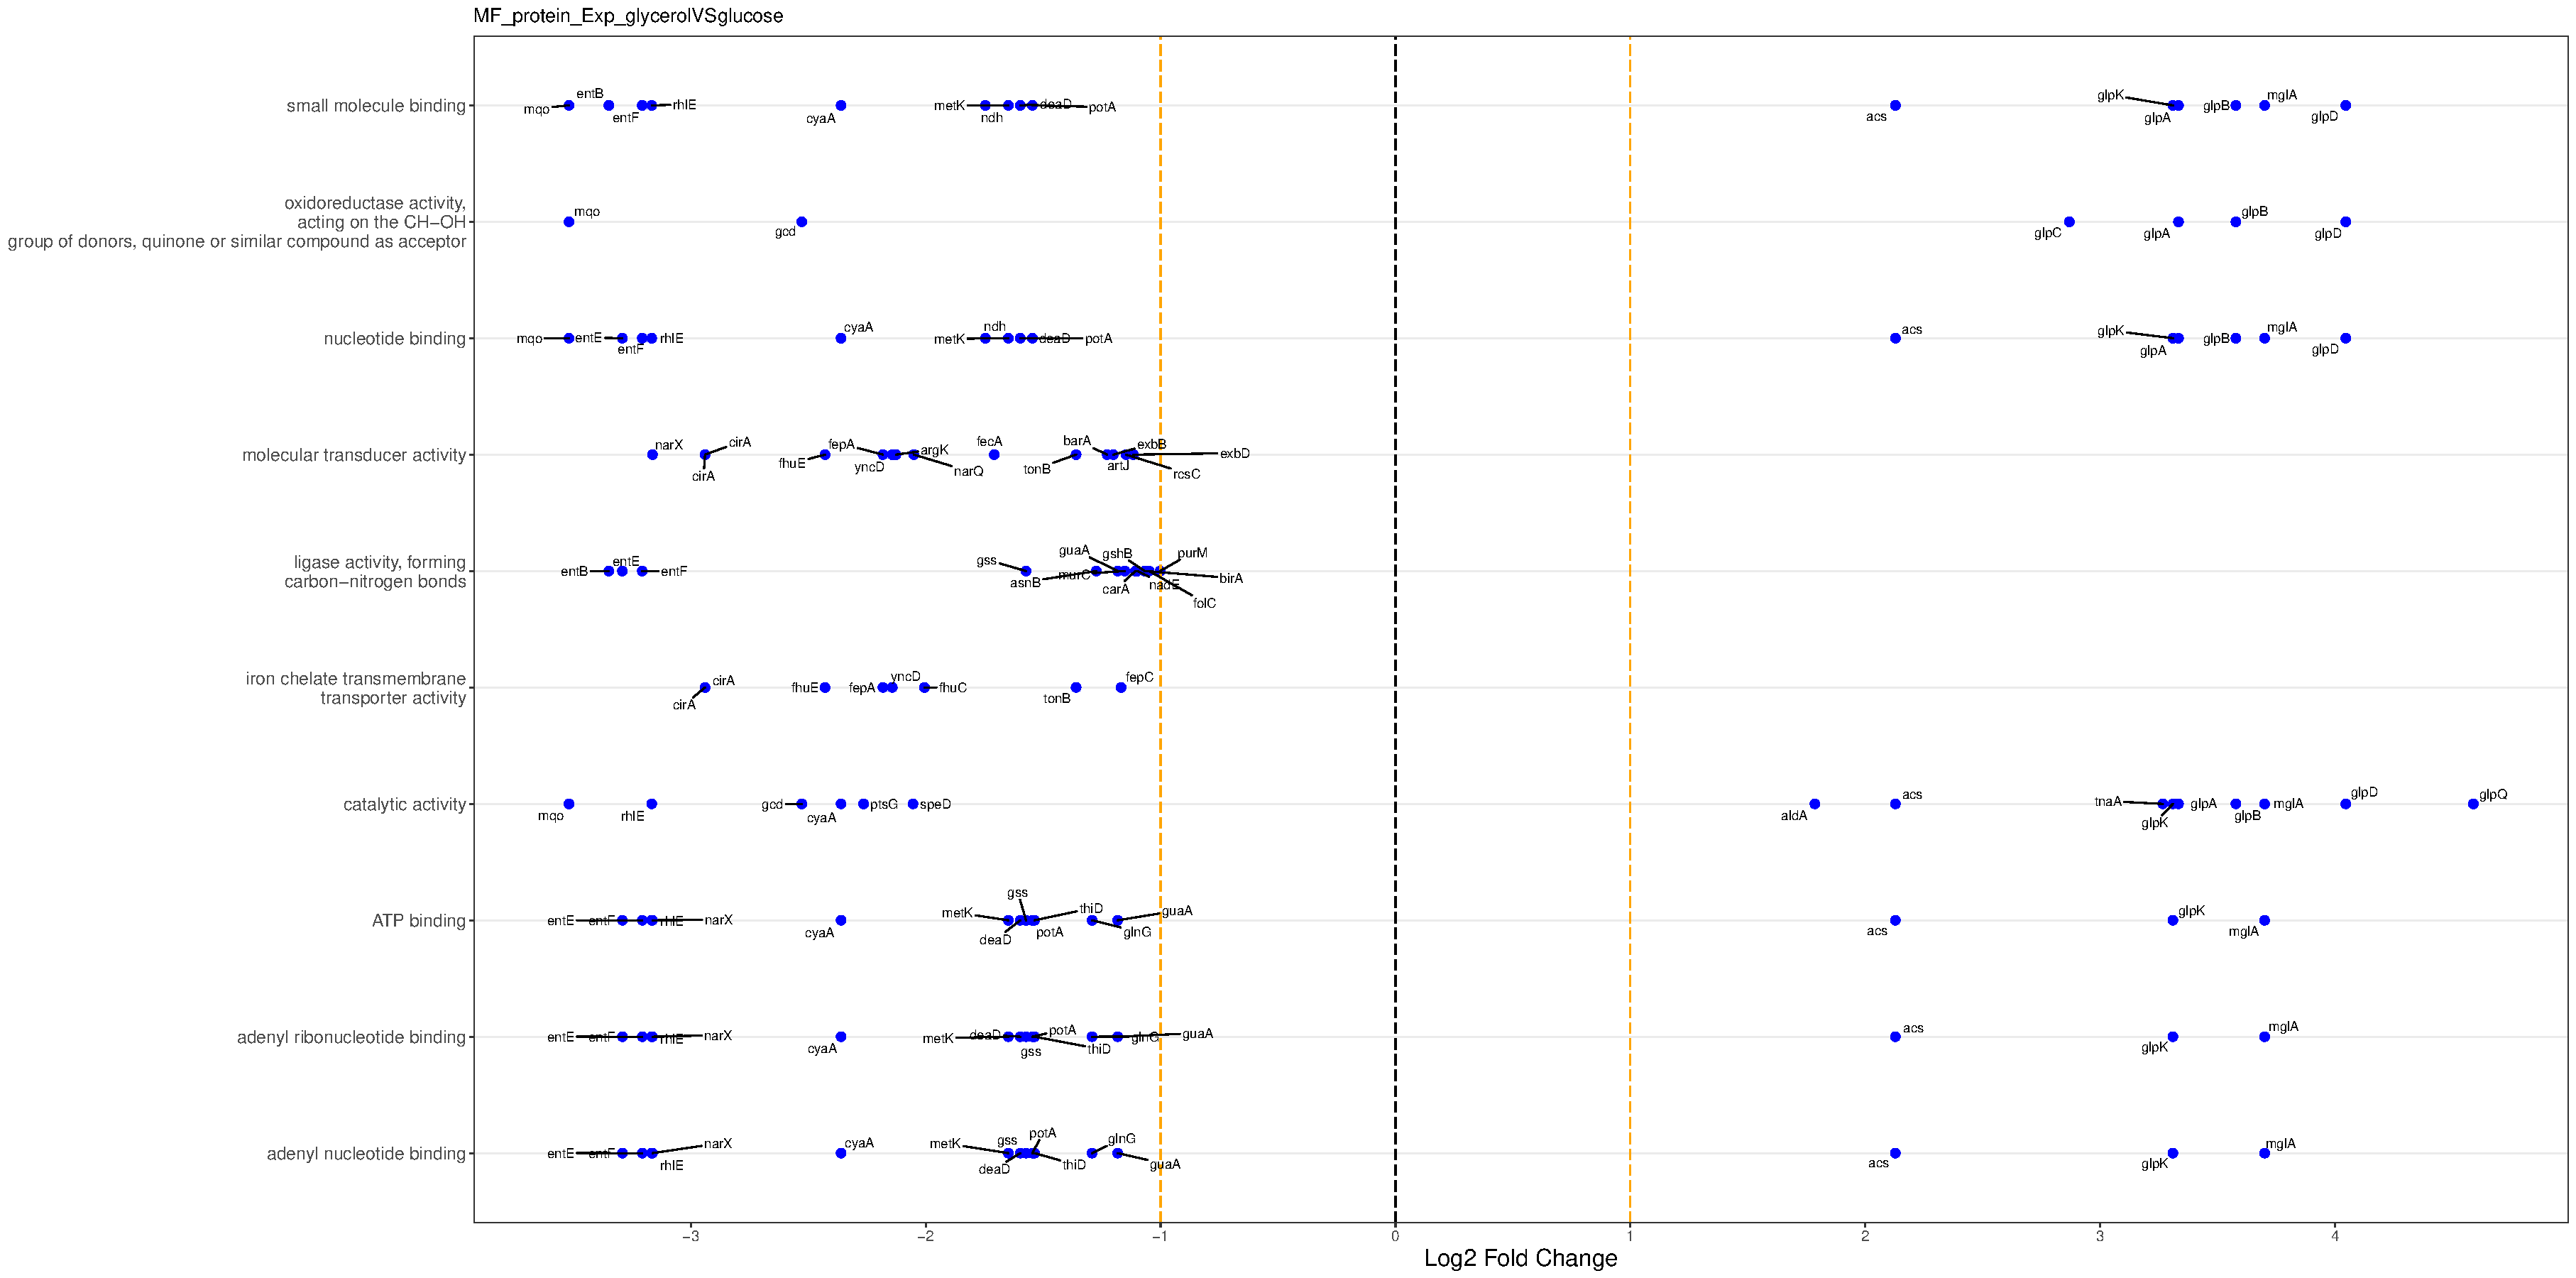
\includegraphics[width=1.0\textwidth]{../../d_figures/MF04_protein_Exp_glycerolVSglucose_withTitle.pdf}
	\caption[Significantly differentially expressed GO annotations associated with molecular functions for protein samples in exponential phase tested for glycerol against glucose]
	{\textbf{Significantly differentially expressed GO annotations related with molecular functions and associated genes with glycerol as carbon source, as determined by protein abundances in exponential phase.} The top 10 differentially expressed molecular functions are shown along the $y$ axis, and the relative fold change of the corresponding genes is shown along the $x$ axis. We show up to 10 of the most significantly changed molecular functions and for each molecular function, we show up to 15 of the most significantly changing genes.}
\end{figure}


\begin{figure}[!htb]
	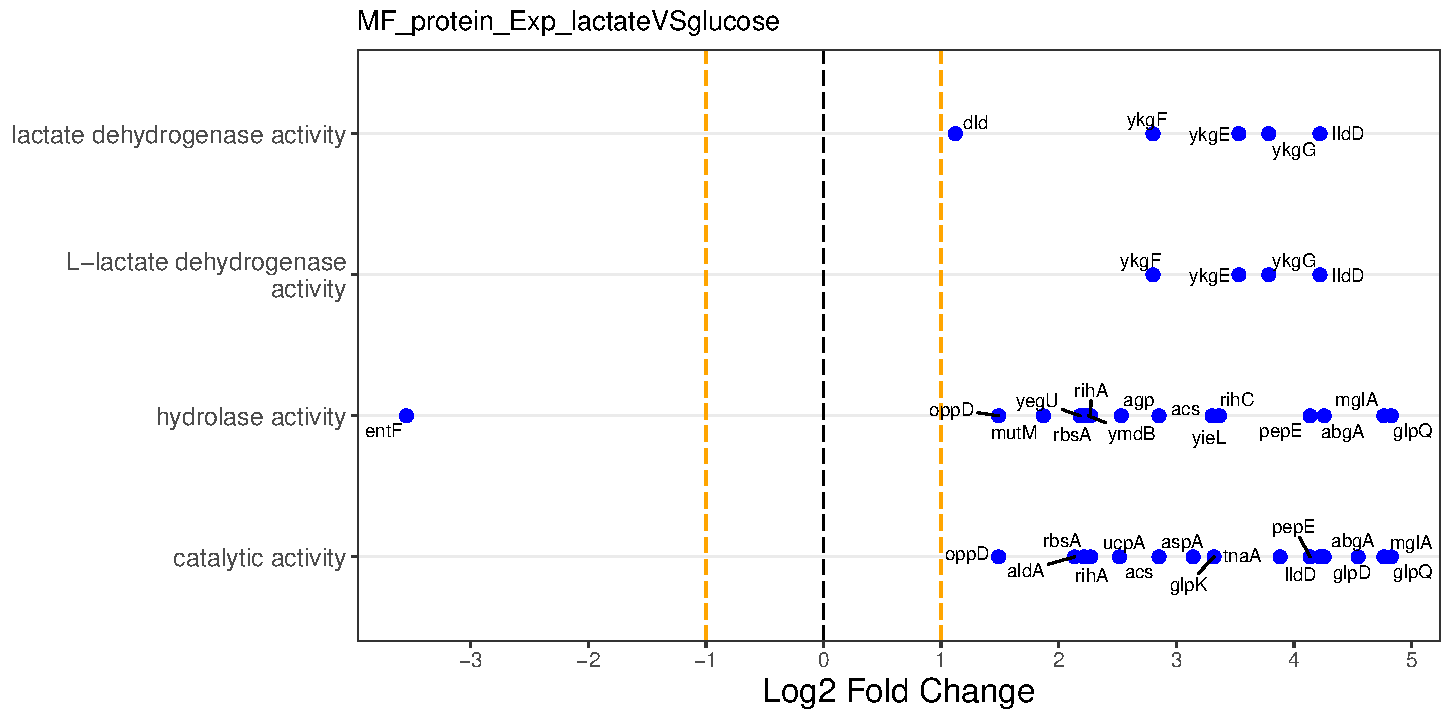
\includegraphics[width=1.0\textwidth]{../../d_figures/MF05_protein_Exp_lactateVSglucose_withTitle.pdf}
	\caption[Significantly differentially expressed GO annotations associated with molecular functions for protein samples in exponential phase tested for lactate against glucose]
	{\textbf{Significantly differentially expressed GO annotations related with molecular functions and associated genes with lactate as carbon source, as determined by protein abundances in exponential phase.} The top 4 differentially expressed molecular functions are shown along the $y$ axis, and the relative fold change of the corresponding genes is shown along the $x$ axis. We show up to 10 of the most significantly changed molecular functions and for each molecular function, we show up to 15 of the most significantly changing genes.}
\end{figure}


\begin{figure}[!htb]
	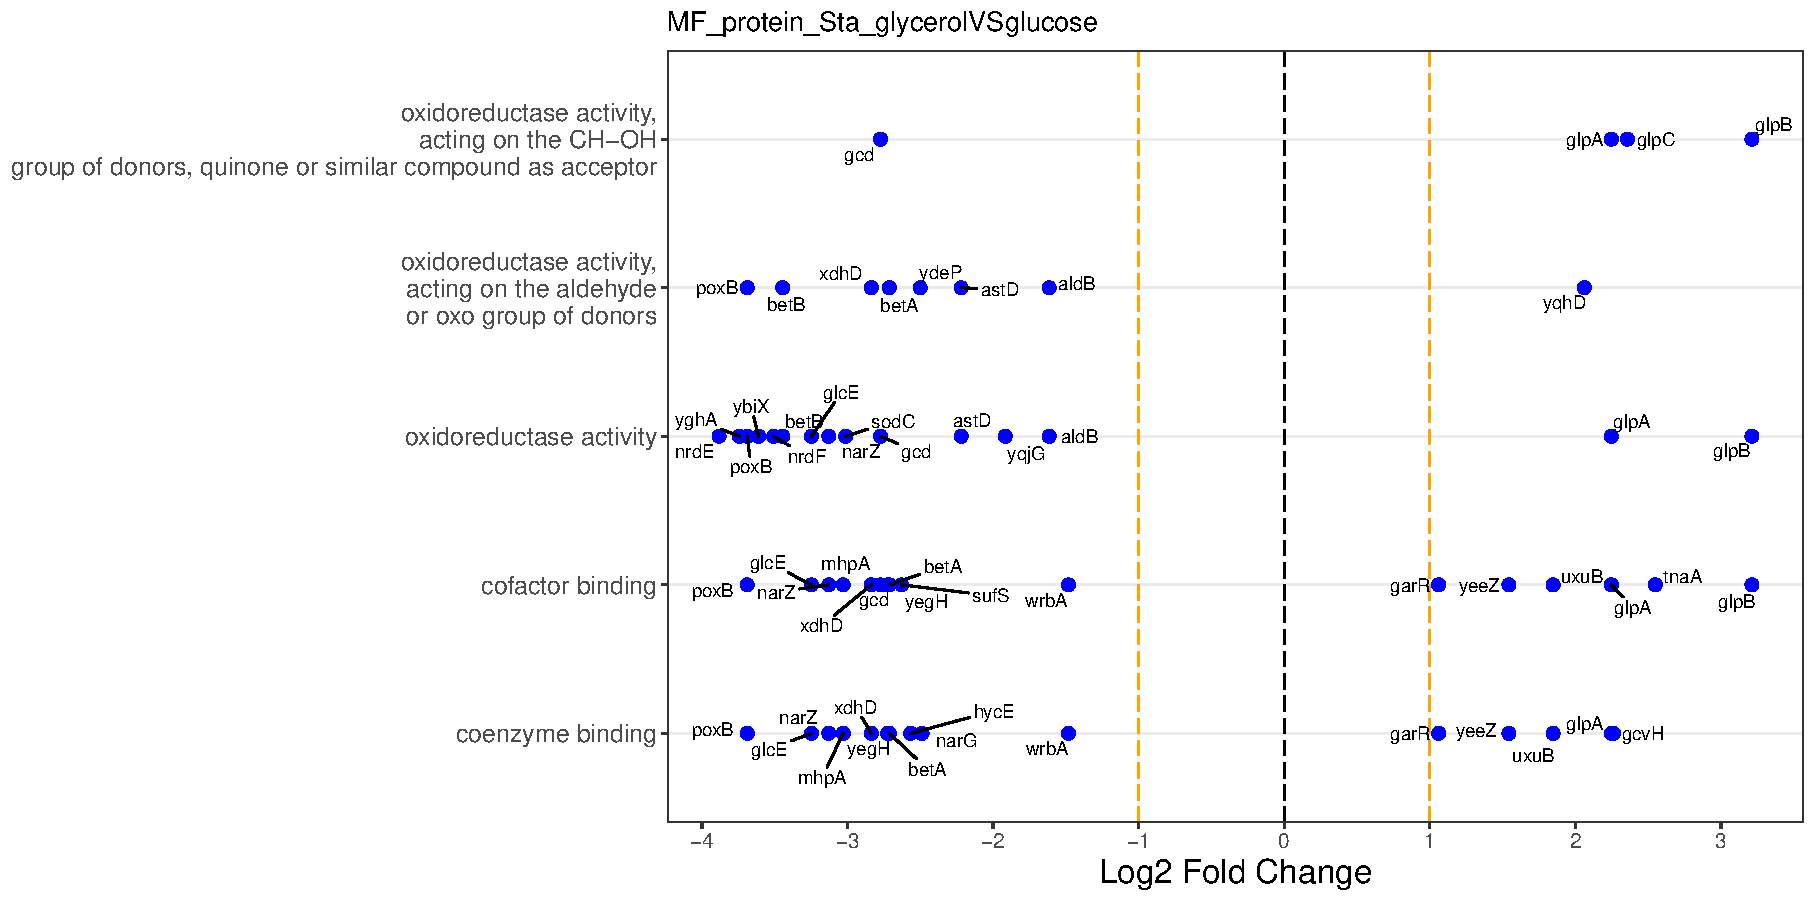
\includegraphics[width=1.0\textwidth]{../../d_figures/MF06_protein_Sta_glycerolVSglucose_withTitle.pdf}
	\caption[Significantly differentially expressed GO annotations associated with molecular functions for protein samples in stationary phase tested for glycerol against glucose]
	{\textbf{Significantly differentially expressed GO annotations related with molecular functions and associated genes with glycerol as carbon source, as determined by protein abundances in stationary phase.} The top 5 differentially expressed molecular functions are shown along the $y$ axis, and the relative fold change of the corresponding genes is shown along the $x$ axis. We show up to 10 of the most significantly changed molecular functions and for each molecular function, we show up to 15 of the most significantly changing genes.}
\end{figure}

\begin{figure}[!htb]
	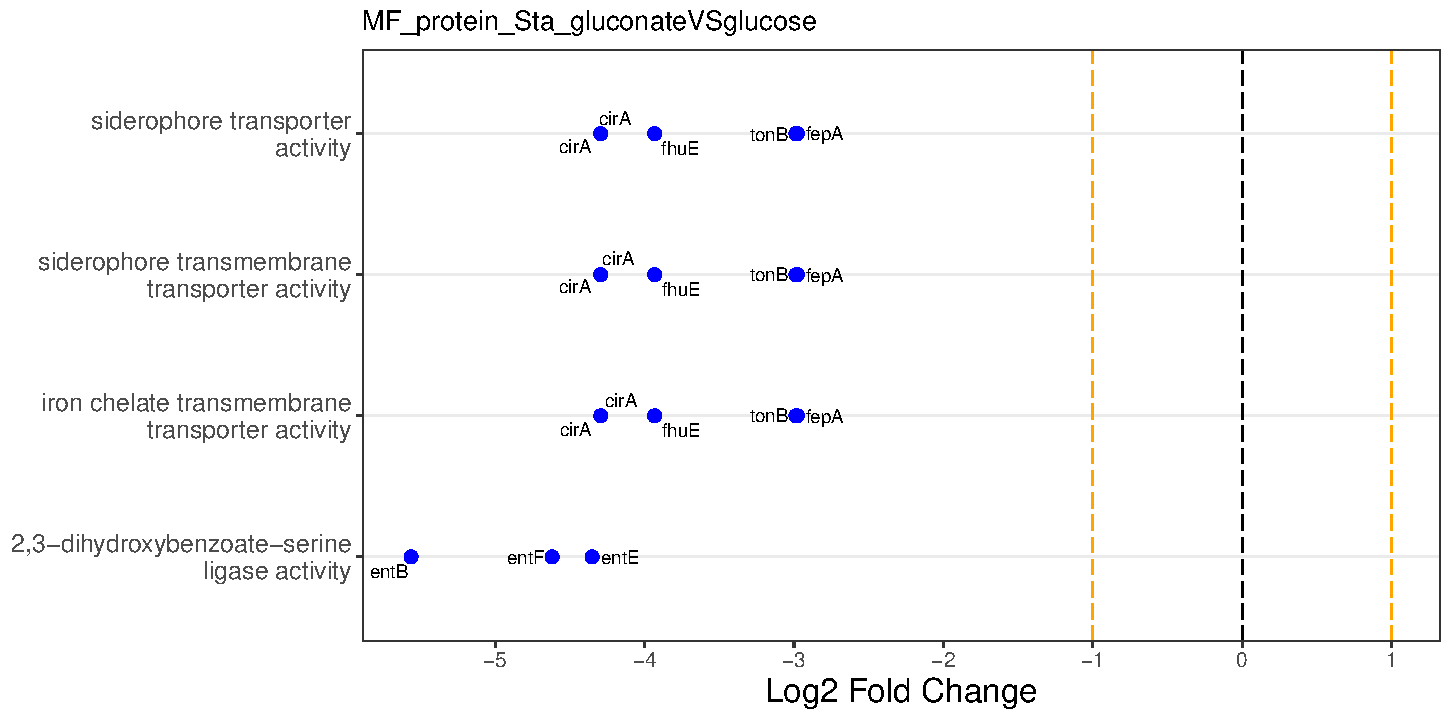
\includegraphics[width=1.0\textwidth]{../../d_figures/MF07_protein_Sta_gluconateVSglucose_withTitle.pdf}
	\caption[Significantly differentially expressed GO annotations associated with molecular functions for protein samples in stationary phase tested for gluconate against glucose]
	{\textbf{Significantly differentially expressed GO annotations related with molecular functions and associated genes with gluconate as carbon source, as determined by protein abundances in stationary phase.} The top 4 differentially expressed molecular functions are shown along the $y$ axis, and the relative fold change of the corresponding genes is shown along the $x$ axis. We show up to 10 of the most significantly changed molecular functions and for each molecular function, we show up to 15 of the most significantly changing genes.}
\end{figure}

\begin{figure}[!htb]
	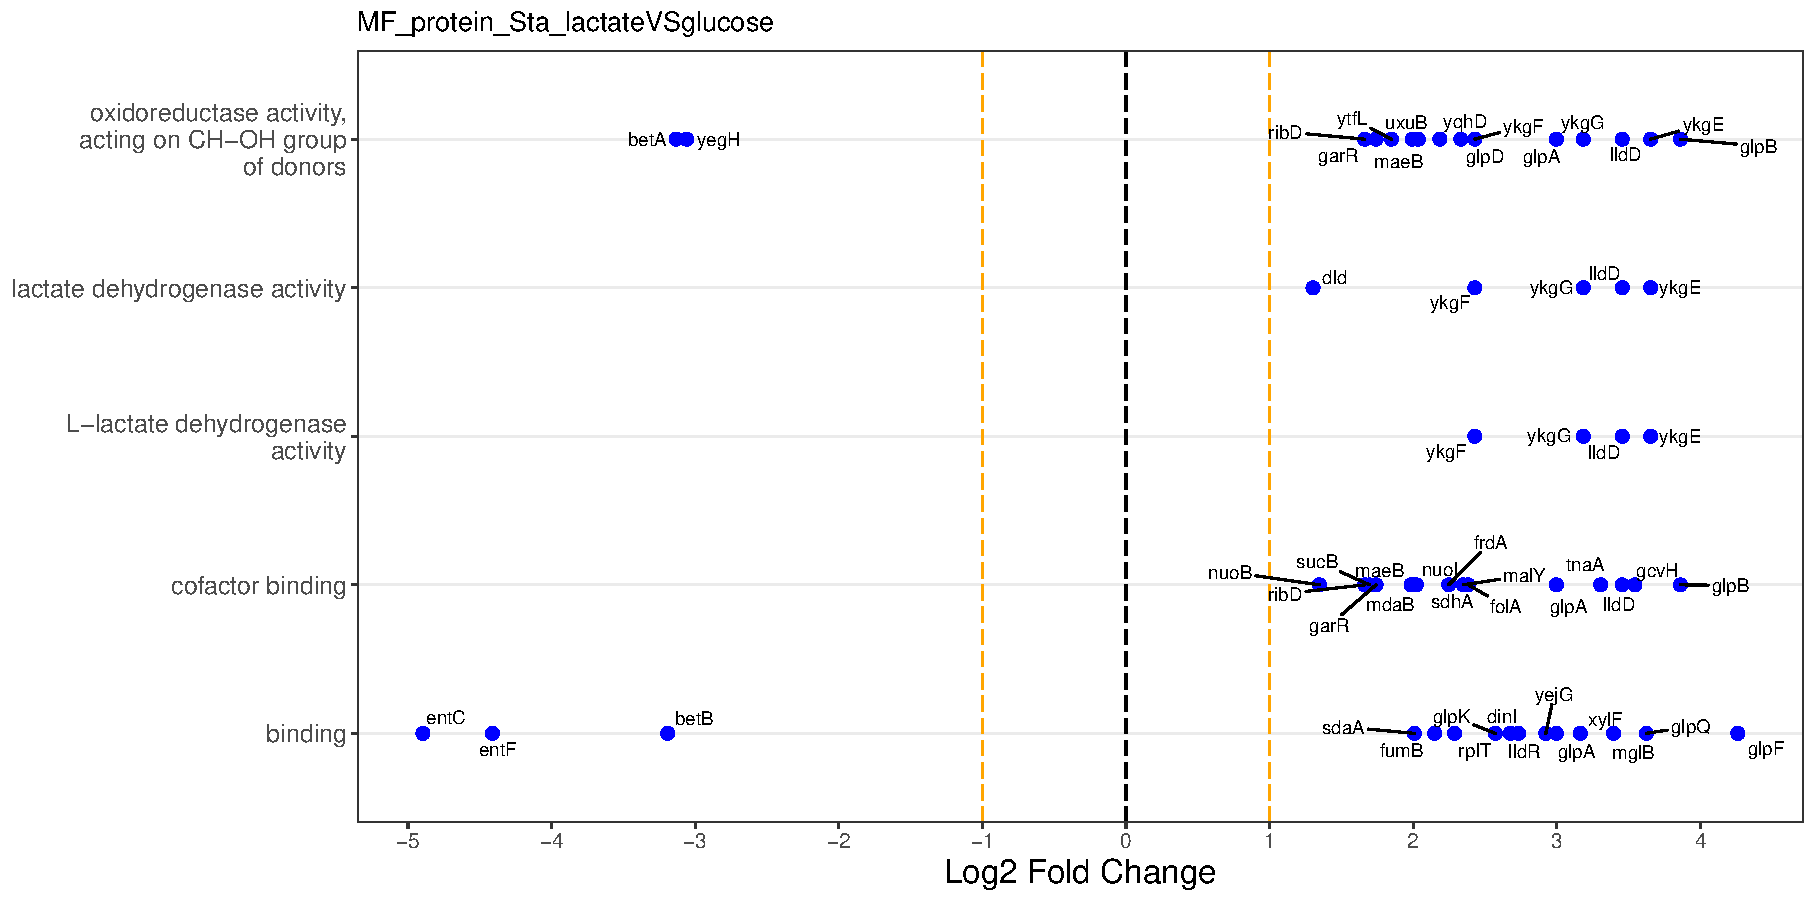
\includegraphics[width=1.0\textwidth]{../../d_figures/MF08_protein_Sta_lactateVSglucose_withTitle.pdf}
	\caption[Significantly differentially expressed GO annotations associated with molecular functions for protein samples in stationary phase tested for lactate against glucose]
	{\textbf{Significantly differentially expressed GO annotations related with molecular functions and associated genes with lactate as carbon source, as determined by protein abundances in stationary phase.} The top 5 differentially expressed molecular functions are shown along the $y$ axis, and the relative fold change of the corresponding genes is shown along the $x$ axis. We show up to 10 of the most significantly changed molecular functions and for each molecular function, we show up to 15 of the most significantly changing genes.}
\end{figure}

\begin{figure}[!htb]
	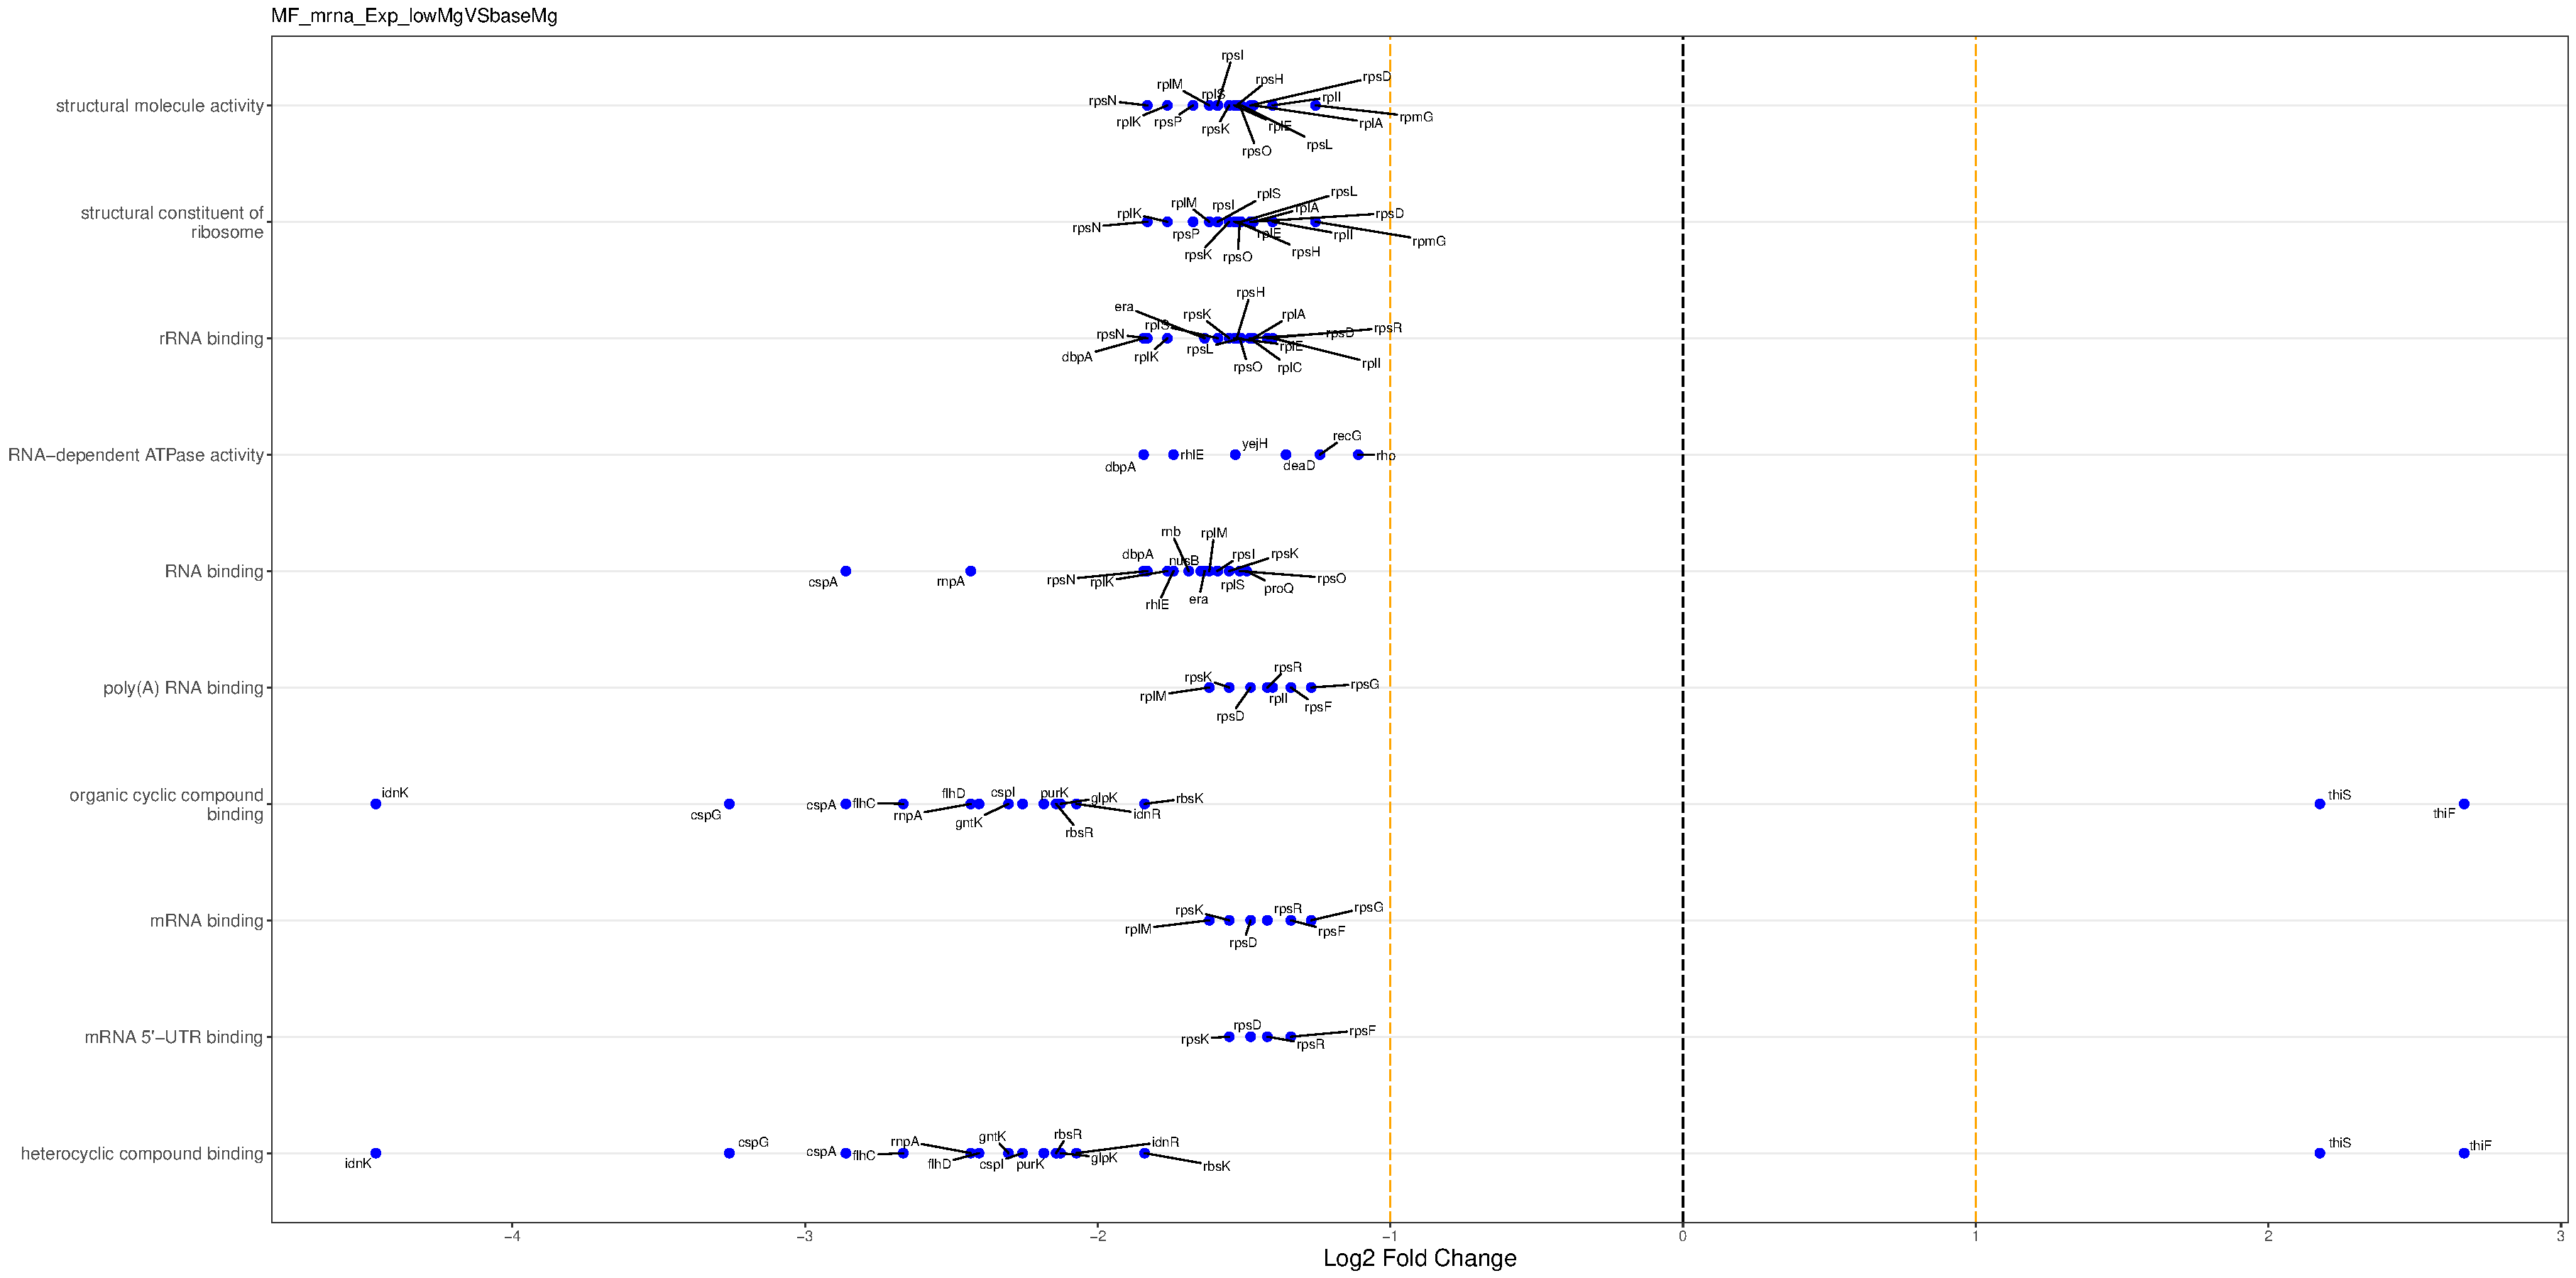
\includegraphics[width=1.0\textwidth]{../../d_figures/MF09_mrna_Exp_lowMgVSbaseMg_withTitle.pdf}
	\caption[Significantly differentially expressed GO annotations associated with molecular functions for mRNA samples in exponential phase tested for low Mg\textsuperscript{2+} levels against base Mg\textsuperscript{2+} levels]
	{\textbf{Significantly differentially expressed GO annotations related with molecular functions and associated genes with low Mg\textsuperscript{2+} levels, as determined by mRNA abundances in exponential phase.} The top 10 differentially expressed molecular functions are shown along the $y$ axis, and the relative fold change of the corresponding genes is shown along the $x$ axis. We show up to 10 of the most significantly changed molecular functions and for each molecular function, we show up to 15 of the most significantly changing genes.}
\end{figure}

\begin{figure}[!htb]
	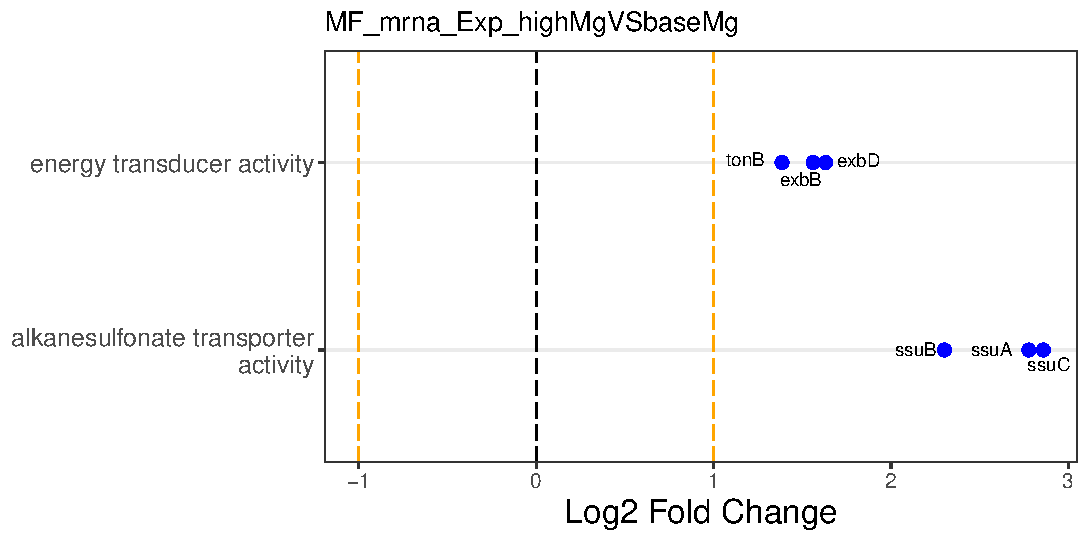
\includegraphics[width=1.0\textwidth]{../../d_figures/MF10_mrna_Exp_highMgVSbaseMg_withTitle.pdf}
	\caption[Significantly differentially expressed GO annotations associated with molecular functions for mRNA samples in exponential phase tested for high Mg\textsuperscript{2+} levels against base Mg\textsuperscript{2+} levels]
	{\textbf{Significantly differentially expressed GO annotations related with molecular functions and associated genes with high Mg\textsuperscript{2+} levels, as determined by mRNA abundances in exponential phase.} The top 3 differentially expressed molecular functions are shown along the $y$ axis, and the relative fold change of the corresponding genes is shown along the $x$ axis. We show up to 10 of the most significantly changed molecular functions and for each molecular function, we show up to 15 of the most significantly changing genes.}
\end{figure}

\begin{figure}[!htb]
	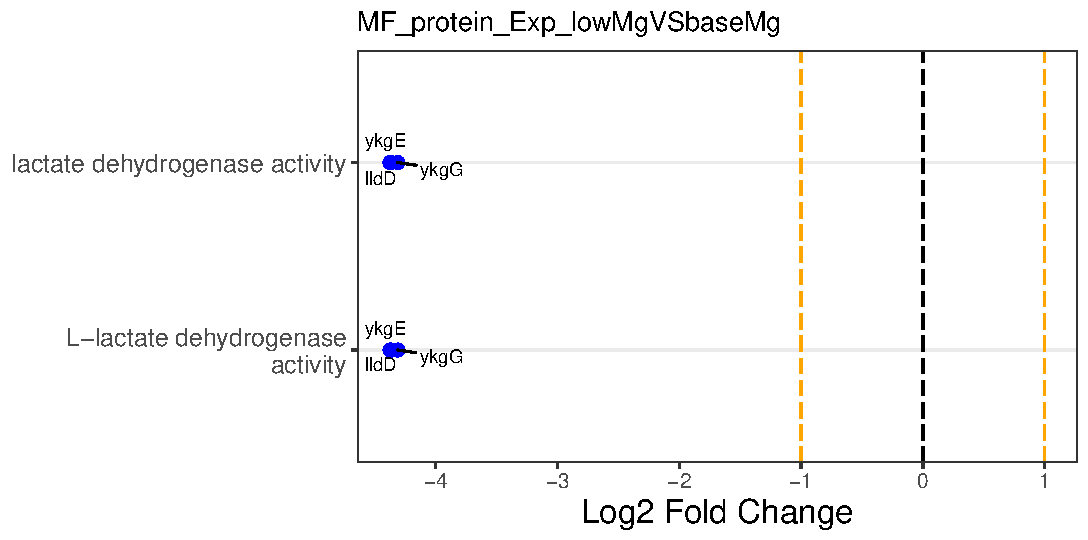
\includegraphics[width=1.0\textwidth]{../../d_figures/MF11_protein_Exp_lowMgVSbaseMg_withTitle.pdf}
	\caption[Significantly differentially expressed GO annotations associated with molecular functions for protein samples in exponential phase tested for low Mg\textsuperscript{2+} levels against base Mg\textsuperscript{2+} levels]
	{\textbf{Significantly differentially expressed GO annotations related with molecular functions and associated genes with low Mg\textsuperscript{2+} levels, as determined by protein abundances in exponential phase.} The top 2 differentially expressed molecular functions are shown along the $y$ axis, and the relative fold change of the corresponding genes is shown along the $x$ axis. We show up to 10 of the most significantly changed molecular functions and for each molecular function, we show up to 15 of the most significantly changing genes.}
\end{figure}

\begin{figure}[!htb]
	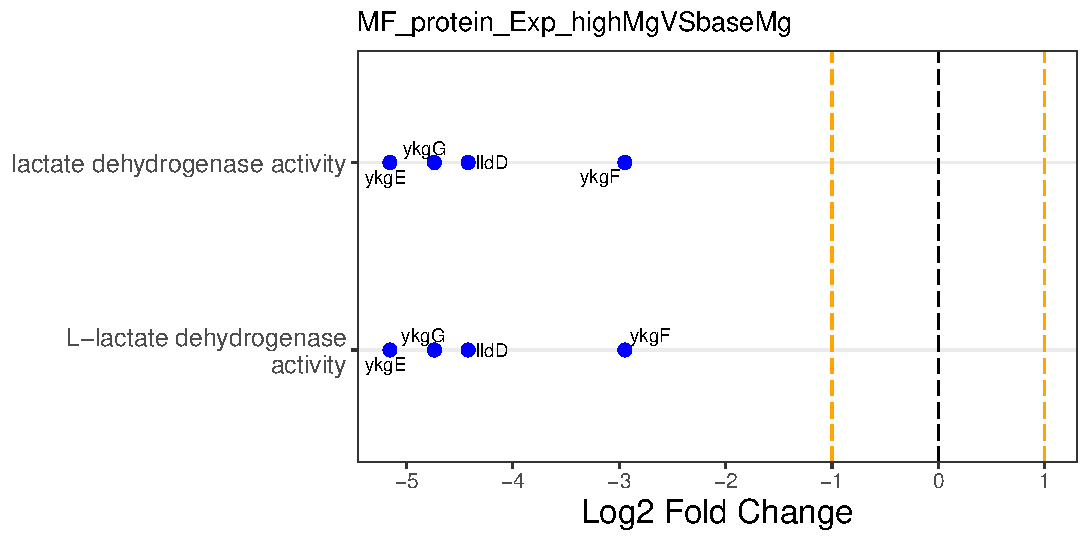
\includegraphics[width=1.0\textwidth]{../../d_figures/MF12_protein_Exp_highMgVSbaseMg_withTitle.pdf}
	\caption[Significantly differentially expressed GO annotations associated with molecular functions for protein samples in exponential phase tested for high Mg\textsuperscript{2+} levels against base Mg\textsuperscript{2+} levels]
	{\textbf{Significantly differentially expressed GO annotations related with molecular functions and associated genes with high Mg\textsuperscript{2+} levels, as determined by protein abundances in exponential phase.} The top 2 differentially expressed molecular functions are shown along the $y$ axis, and the relative fold change of the corresponding genes is shown along the $x$ axis. We show up to 10 of the most significantly changed molecular functions and for each molecular function, we show up to 15 of the most significantly changing genes.}
\end{figure}

\begin{figure}[!htb]
	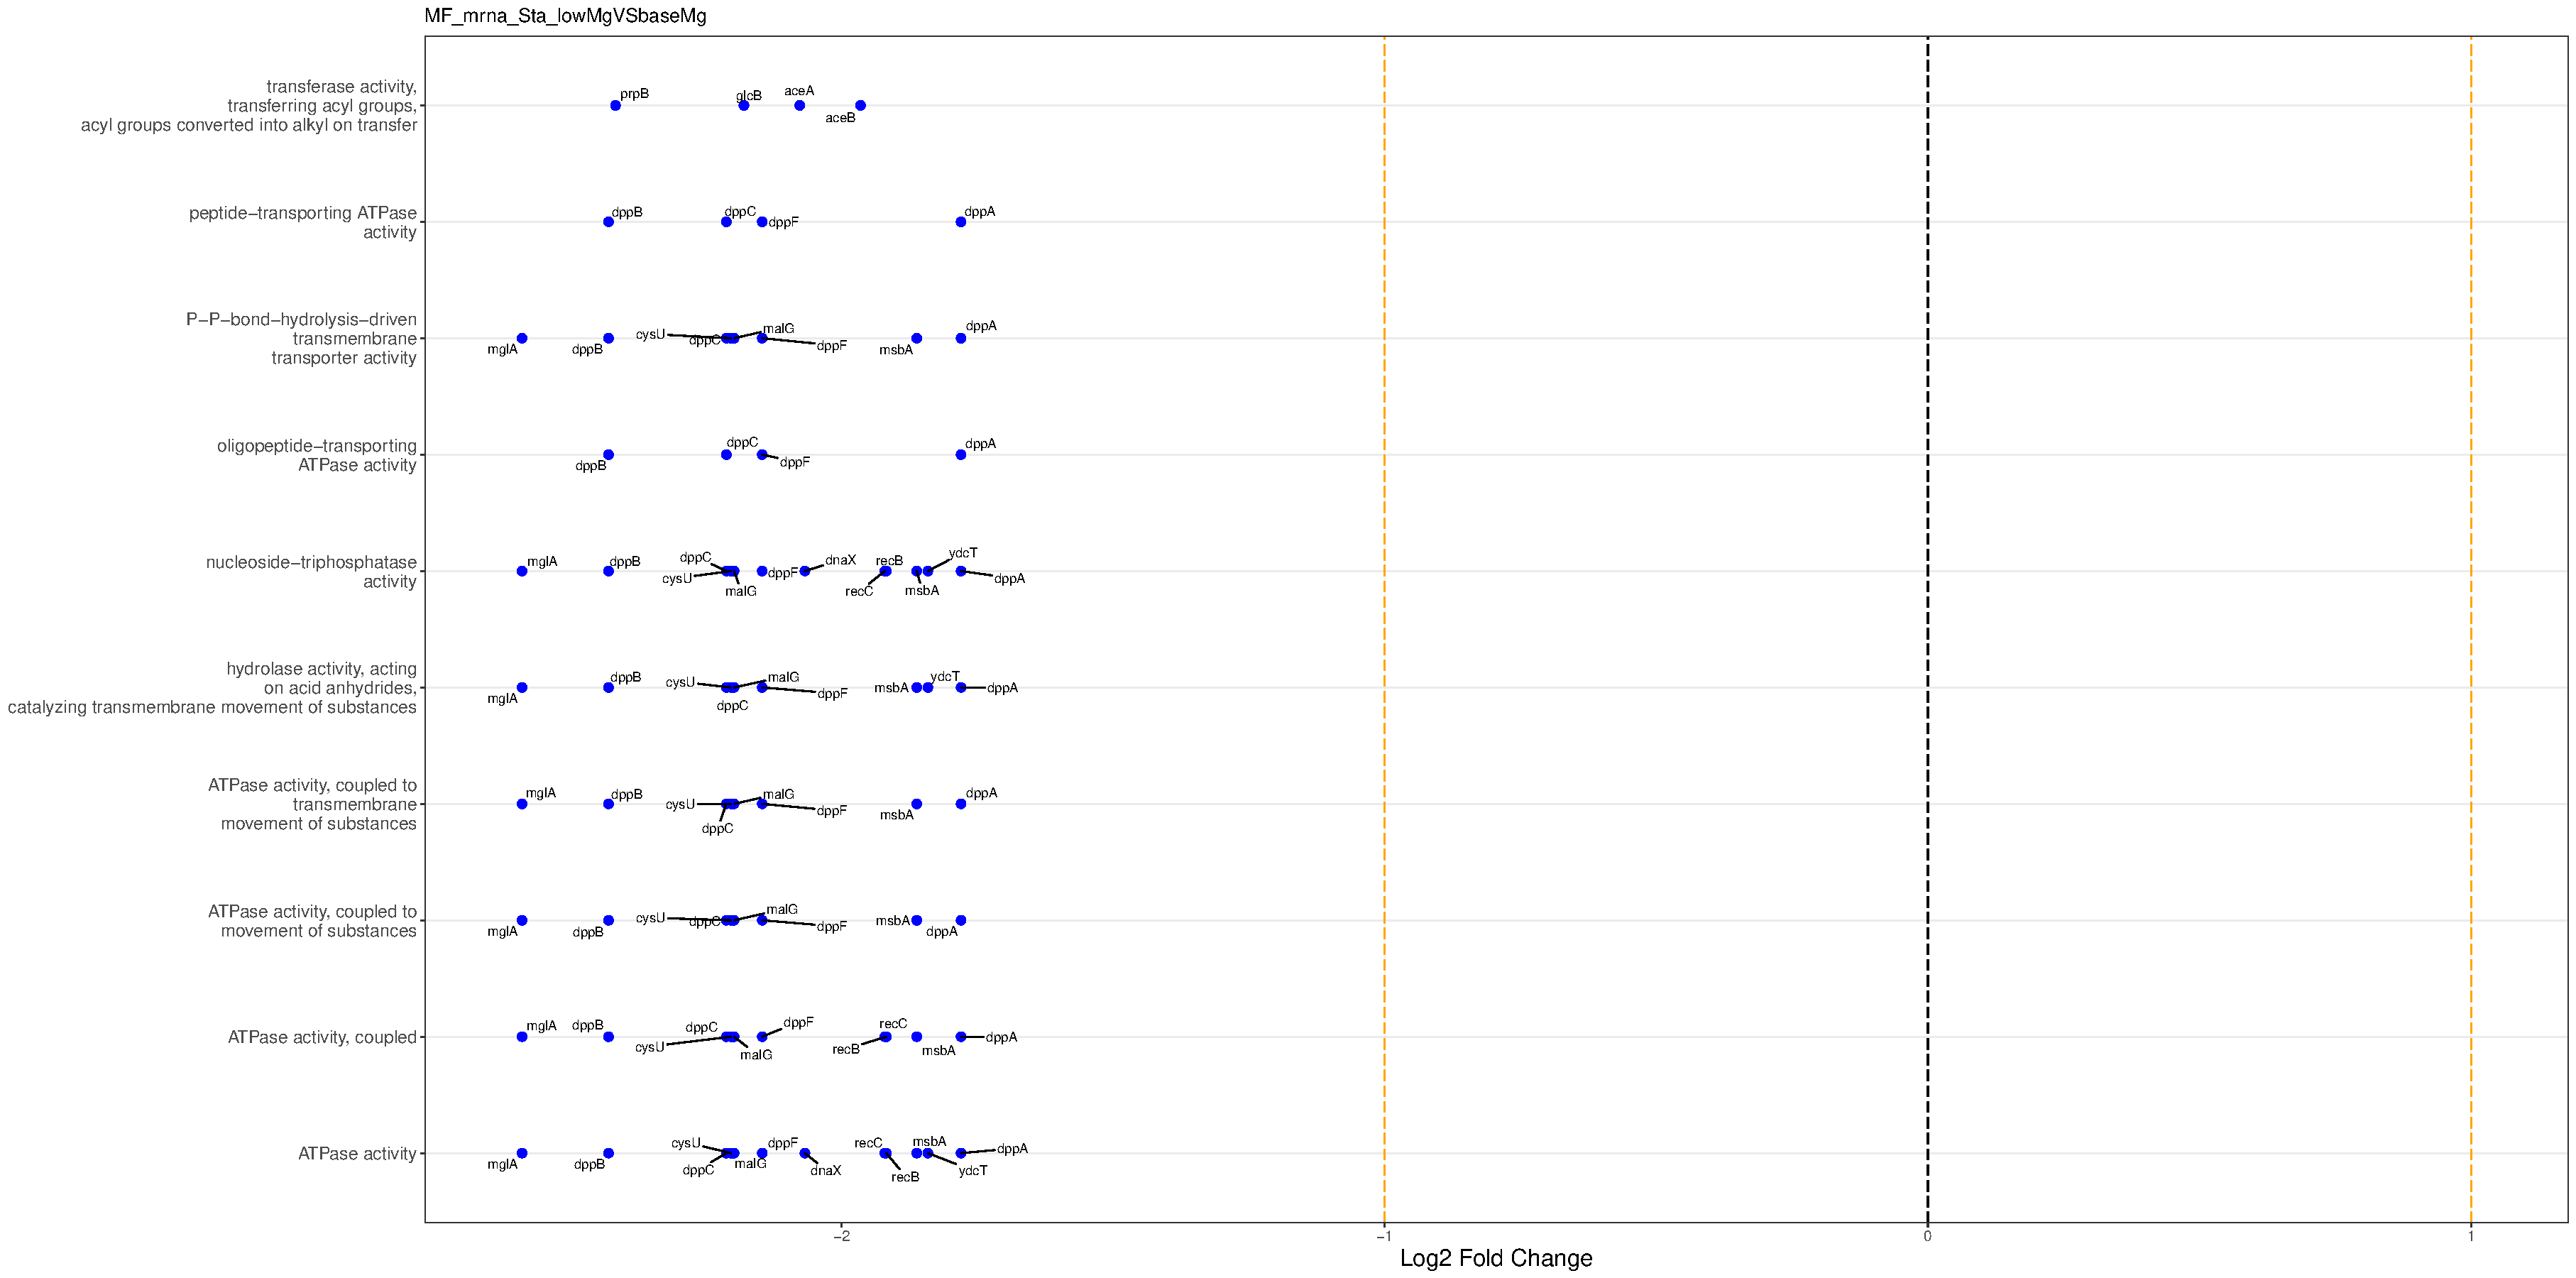
\includegraphics[width=1.0\textwidth]{../../d_figures/MF13_mrna_Sta_lowMgVSbaseMg_withTitle.pdf}
	\caption[Significantly differentially expressed GO annotations associated with molecular functions for mRNA samples in stationary phase tested for low Mg\textsuperscript{2+} levels against base Mg\textsuperscript{2+} levels]
	{\textbf{Significantly differentially expressed GO annotations related with molecular functions and associated genes with low Mg\textsuperscript{2+} levels, as determined by mRNA abundances in stationary phase.} The top 10 differentially expressed molecular functions are shown along the $y$ axis, and the relative fold change of the corresponding genes is shown along the $x$ axis. We show up to 10 of the most significantly changed molecular functions and for each molecular function, we show up to 15 of the most significantly changing genes.}
\end{figure}

\begin{figure}[!htb]
	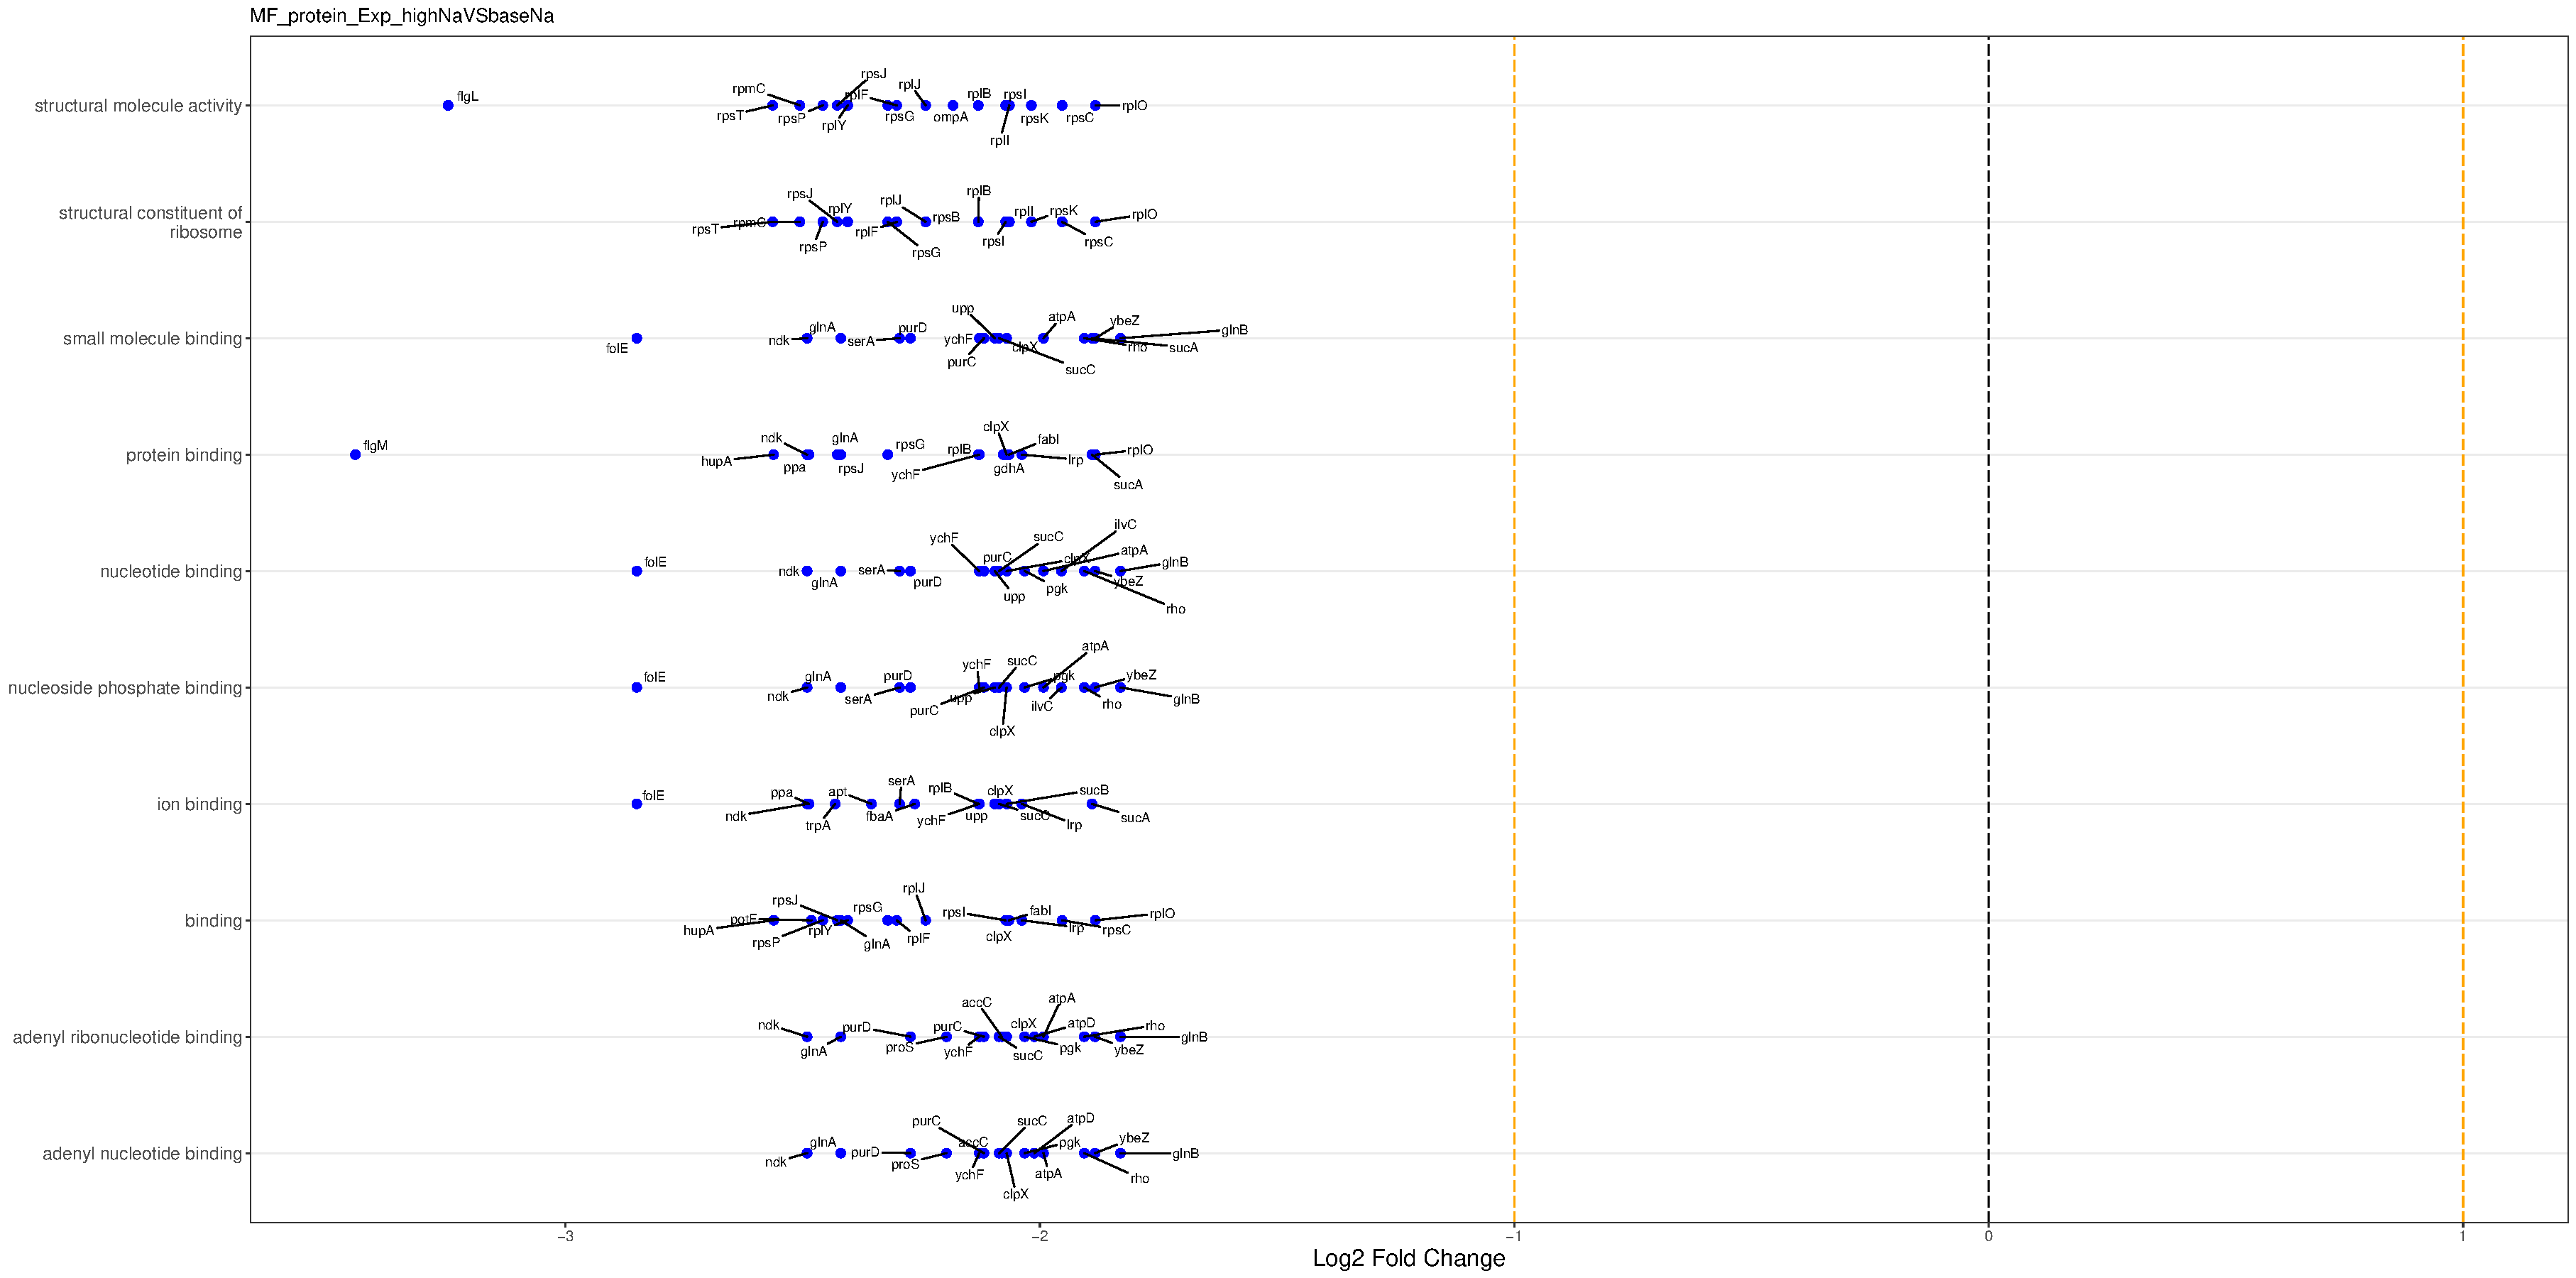
\includegraphics[width=1.0\textwidth]{../../d_figures/MF14_protein_Exp_highNaVSbaseNa_withTitle.pdf}
	\caption[Significantly differentially expressed GO annotations associated with molecular functions for protein samples in exponential phase tested for high Na\textsuperscript{+} levels against base Na\textsuperscript{+} levels]
	{\textbf{Significantly differentially expressed GO annotations related with molecular functions and associated genes with high Na\textsuperscript{+} levels, as determined by protein abundances in exponential phase.} The top differentially expressed molecular functions are shown along the $y$ axis, and the relative fold change of the corresponding genes is shown along the $x$ axis. We show up to 10 of the most significantly changed molecular functions and for each molecular function, we show up to 15 of the most significantly changing genes.}
\end{figure}

\begin{figure}[!htb]
	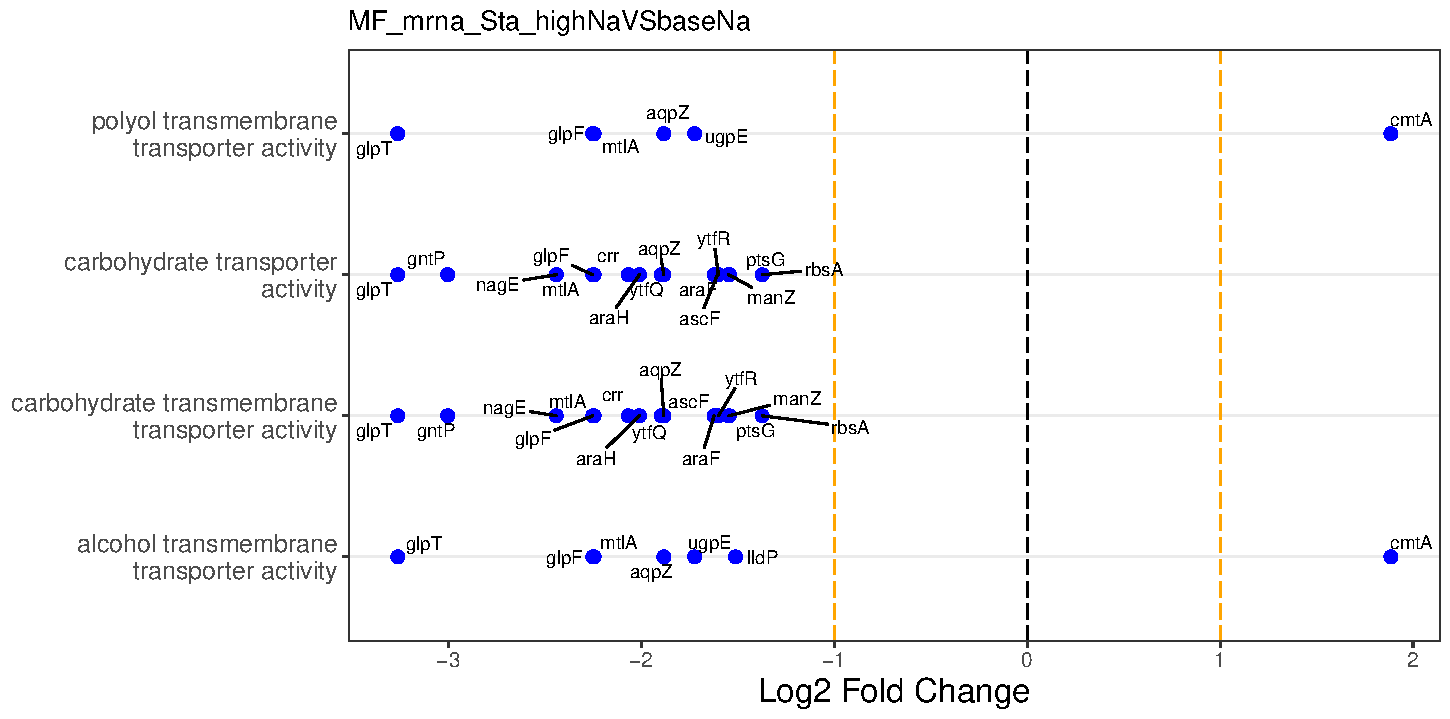
\includegraphics[width=1.0\textwidth]{../../d_figures/MF15_mrna_Sta_highNaVSbaseNa_withTitle.pdf}
	\caption[Significantly differentially expressed GO annotations associated with molecular functions for mRNA samples in stationary phase tested for high Na\textsuperscript{+} levels against base Na\textsuperscript{+} levels]
	{\textbf{Significantly differentially expressed GO annotations related with molecular functions and associated genes with high Na\textsuperscript{+} levels, as determined by mRNA abundances in stationary phase.} The top 5 differentially expressed molecular functions are shown along the $y$ axis, and the relative fold change of the corresponding genes is shown along the $x$ axis. We show up to 10 of the most significantly changed molecular functions and for each molecular function, we show up to 15 of the most significantly changing genes.}
\end{figure}

\begin{figure}[!htb]
	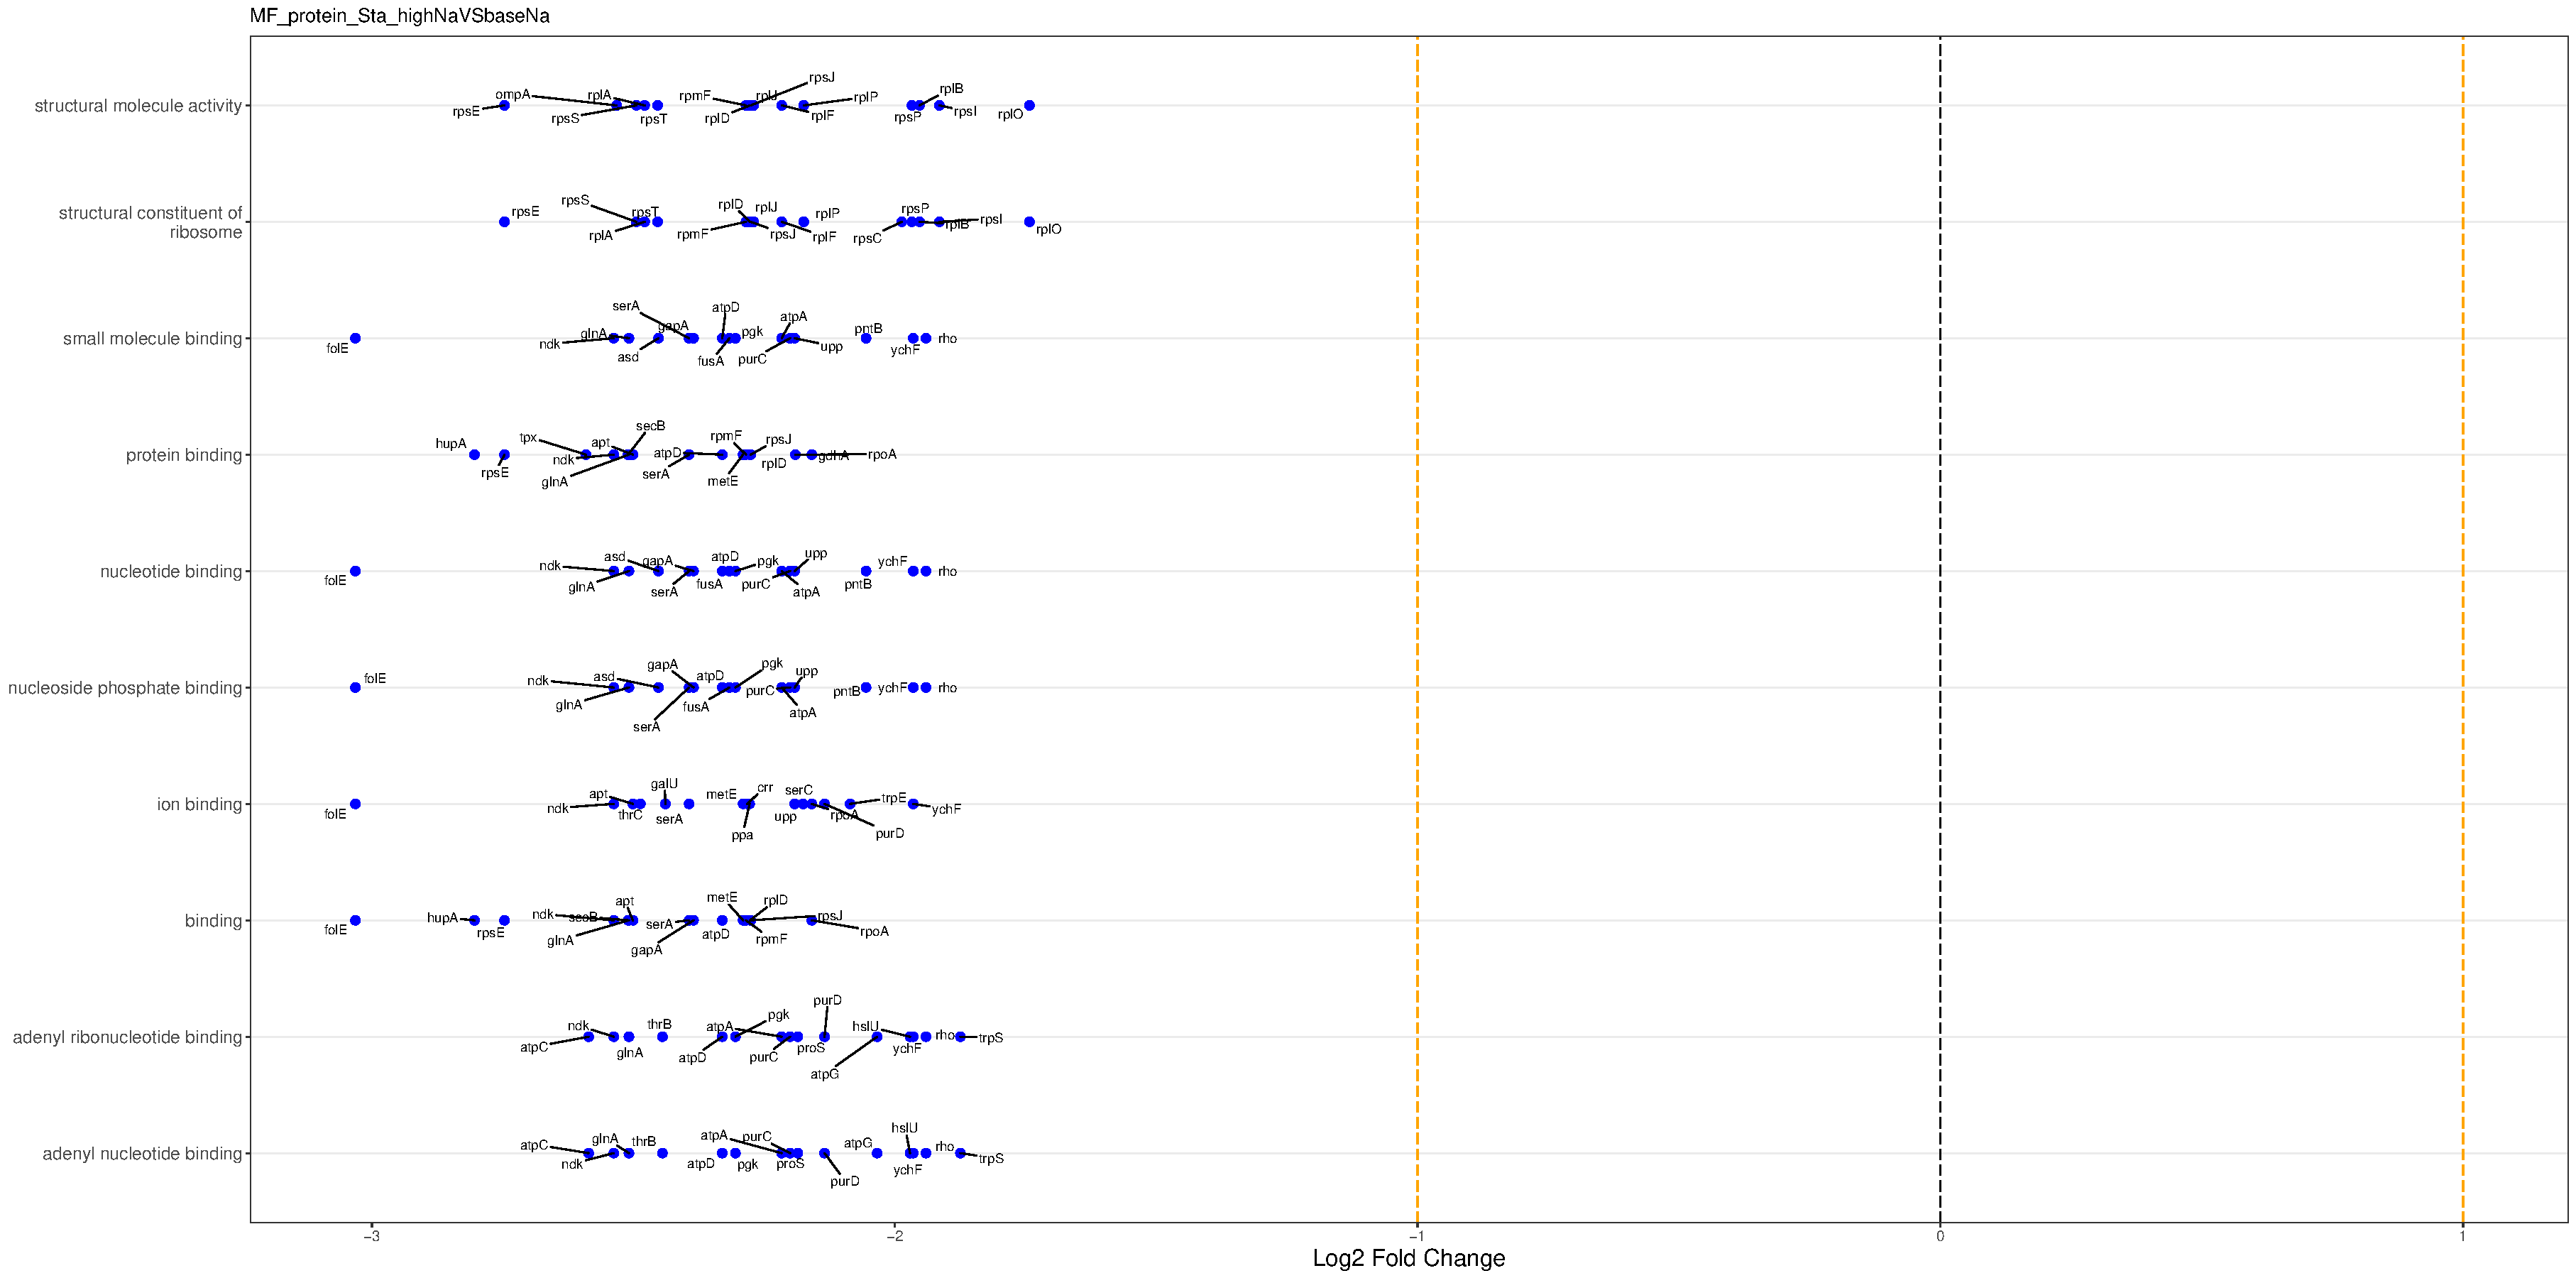
\includegraphics[width=1.0\textwidth]{../../d_figures/MF16_protein_Sta_highNaVSbaseNa_withTitle.pdf}
	\caption[Significantly differentially expressed GO annotations associated with molecular functions for protein samples in stationary phase tested for high Na\textsuperscript{+} levels against base Na\textsuperscript{+} levels]
	{\textbf{Significantly differentially expressed GO annotations related with molecular functions and associated genes with high Na\textsuperscript{+} levels, as determined by protein abundances in stationary phase.} The top 10 differentially expressed molecular functions are shown along the $y$ axis, and the relative fold change of the corresponding genes is shown along the $x$ axis. We show up to 10 of the most significantly changed molecular functions and for each molecular function, we show up to 15 of the most significantly changing genes.}
\end{figure}





\clearpage
\begin{figure}[!htb]
	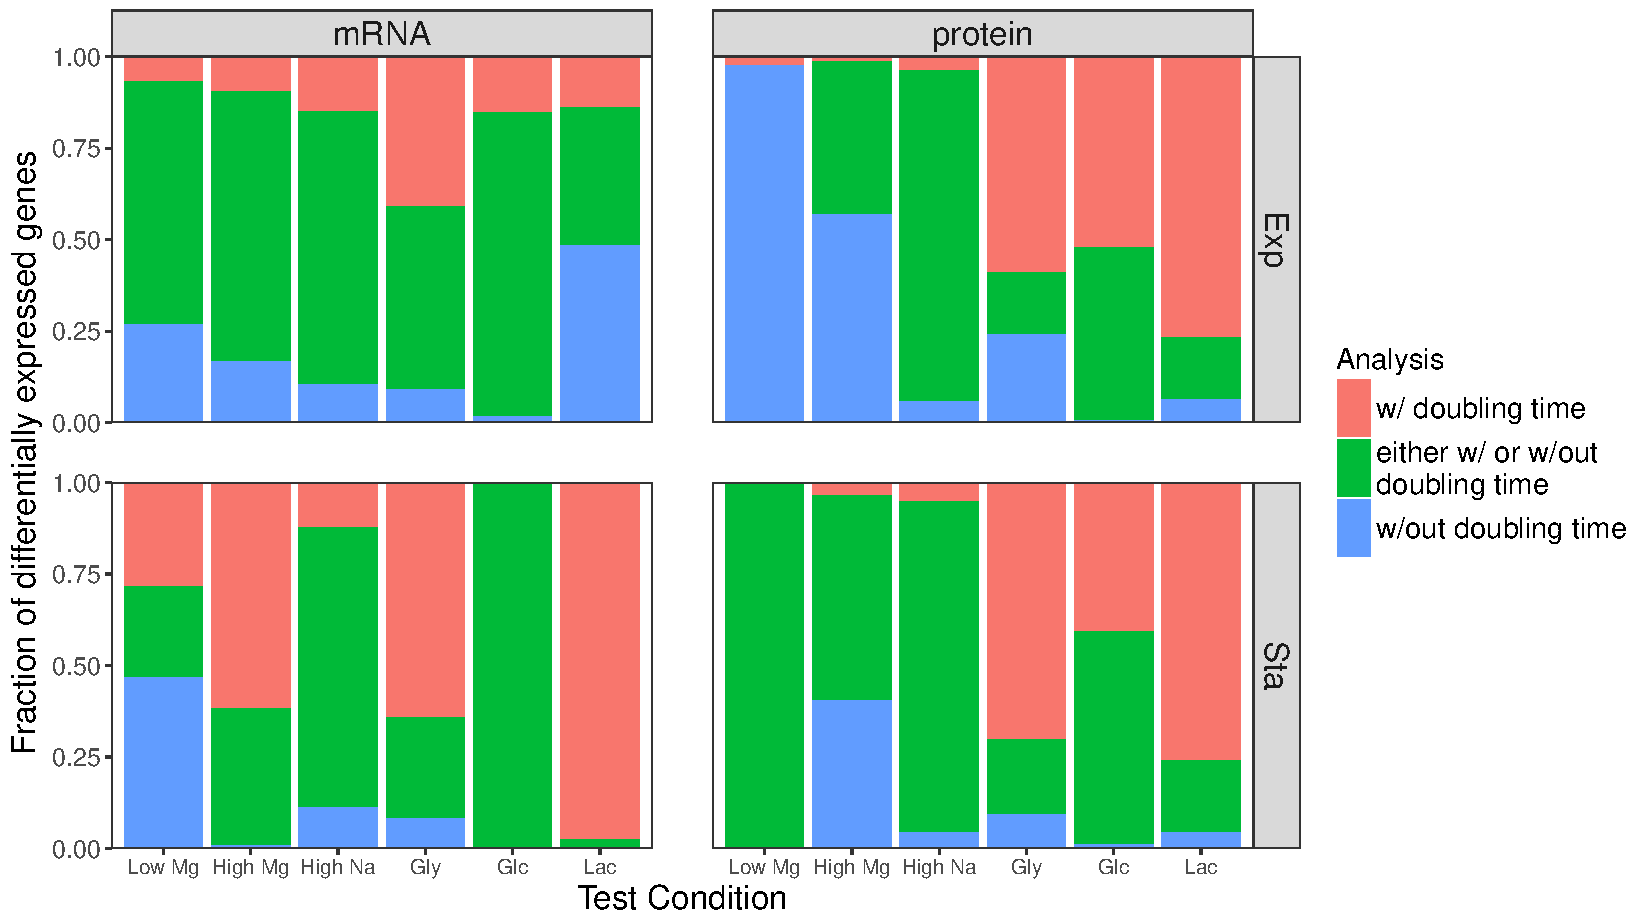
\includegraphics[width=1\textwidth]{../../c_figures/difference_rtw_GrowthControl.pdf}
	\caption[Change in differentially expressed genes between two controls: "batch" vs "batch + doubling time"]
	{\textbf{Change in differentially expressed genes between two controls: "batch" vs "batch + growth rate".} Red represent the fraction of genes that significantly changed only under control of "batch + doubling time". Green represent the fraction of genes appear in both controlling for "batch + doubling time" and for "batch". Blue represents the fraction of genes appear only under control of "batch". As can be seen from figure 5, the full block of red for lactate, mRNA in stationary phase is because of few to none significantly changing genes under control of "batch". Big blocks of red for high Mg\textsuperscript{2+} and glycerol for again mRNA data in stationary phase appeared because of the same reason. On the other hand red blocks for protein data associated with carbon sources for both exponential and stationary phases are meaningful and indicates genes that do not change with growth rate, while the cell is under treated with different carbon sources.}
\end{figure}




\clearpage
\begin{figure}[!htb]
	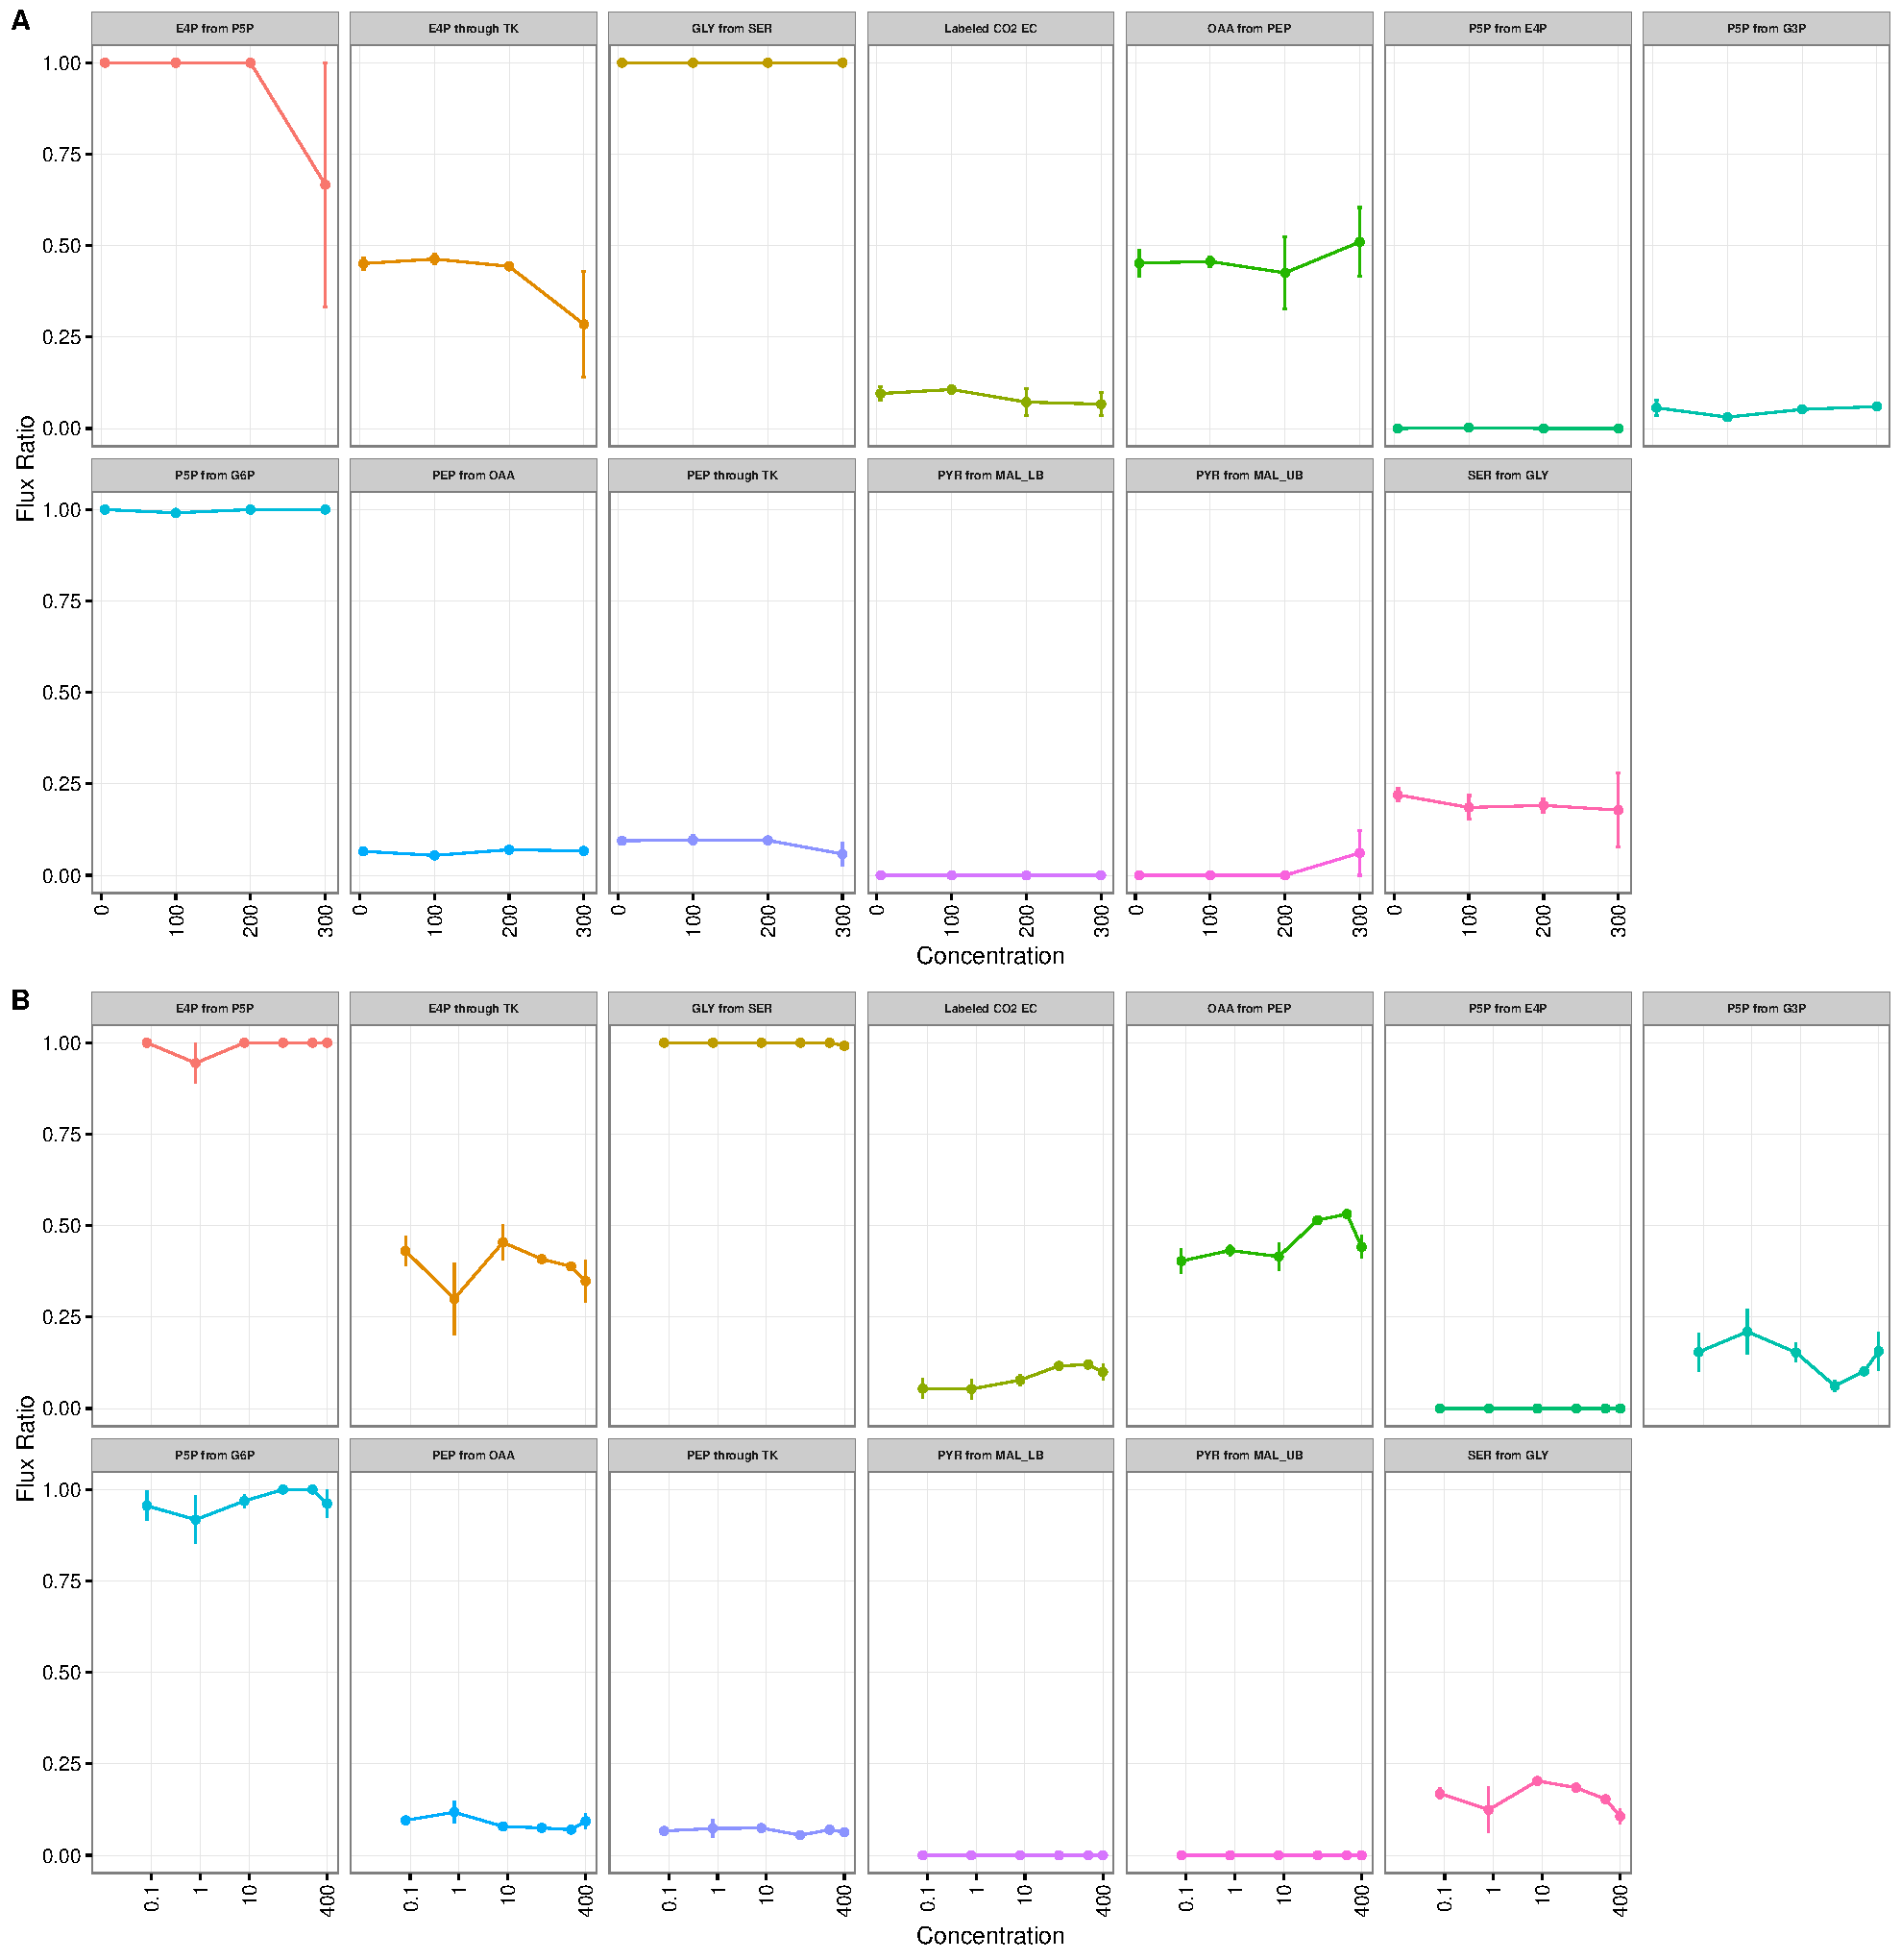
\includegraphics[width=1\textwidth]{../../e_figures/Exp.pdf}
	\caption[Flux ratios versus ion concentrations]
	{\textbf{Flux ratios versus ion concentrations.} 13 different flux ratios were measured with respect to four different Na\textsuperscript{+} and five different Mg\textsuperscript{2+} concentrations. (A) Concentrations with respect to changing Na+ concentrations. (B) Concentrations with respect to changing Mg\textsuperscript{2+} concentrations. There was no significant trend of increase or decrease in flux ratios with respect to either Na\textsuperscript{+} or Mg\textsuperscript{2+} concentrations (Supplementary Table 12).}
\end{figure}


\end{document}
